% Settings for the default beamer theme
\documentclass[english, aspectratio=169]{beamer}
\usepackage[T1]{fontenc}
\usepackage[utf8]{inputenc}
\usepackage{tabularx}
\usepackage{babel}
\usepackage[ruled,vlined]{algorithm2e}
\SetAlgorithmName{Algoritmus}{algoritmus}{List of Algorithms}
\setcounter{secnumdepth}{3}
\setcounter{tocdepth}{3}

\makeatletter

\newcommand\makebeamertitle{\frame{\maketitle}}

% (ERT) argument for the TOC
\AtBeginDocument{%
  \let\origtableofcontents=\tableofcontents
  \def\tableofcontents{\@ifnextchar[{\origtableofcontents}{\gobbletableofcontents}}
  \def\gobbletableofcontents#1{\origtableofcontents}
}

% Theme settings
\usetheme{Frankfurt}
\usecolortheme{default}
\usefonttheme[onlymath]{serif}

% Template settings
\setbeamertemplate{navigation symbols}{}
\setbeamertemplate{blocks}[rounded][shadow=false]
\setbeamertemplate{title page}[default][colsep=-4bp, rounded=true, shadow=false]
\makeatother

\begin{document}

% Title page
\section{Bevezetés}
\title[]{Üzleti Intelligencia}
\subtitle{11. Előadás: Transzformáló architektúrák}
\author[Kuknyó Dániel]{Kuknyó Dániel\\Budapesti Gazdasági Egyetem}
\date{2023/24\\1.félév}
\makebeamertitle

% Table of contents slide
\begin{frame}
\tableofcontents{}
\end{frame}

% Table of contents of the current section
\begin{frame}
\tableofcontents[currentsection]
\end{frame}

\begin{frame}{Visszacsatolásos neurális hálózatok alapjai}
\renewcommand{\arraystretch}{2.}
\begin{tabularx}{\textwidth}{m{4cm}m{5cm}m{5cm}}
\textbf{Alkalmazás} & \textbf{Input} & \textbf{Output} \\
	Beszédfelismerés & 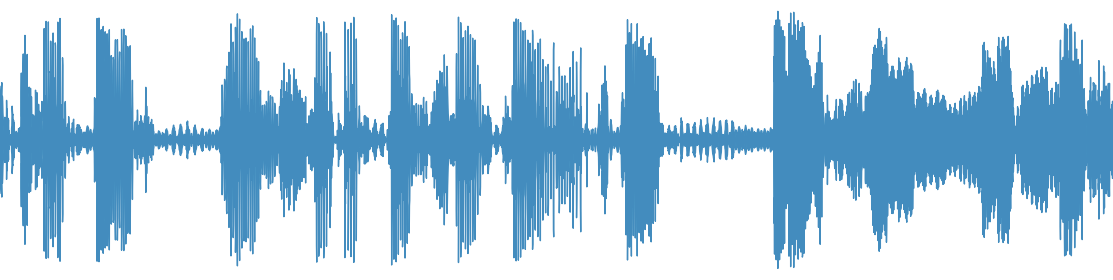
\includegraphics[width=.25\textwidth, keepaspectratio]{../../10_recurrent/doc/images/recurrent_1.png} & "Milyen szép időnk van ma!" \\
	Szemantikai értelmezés & "Ez egy rossz film volt." & 
\includegraphics[width=.2\textwidth, keepaspectratio]{../../10_recurrent/doc/images/recurrent_2.png} \\
	DNS szekvencia elemzés & AGCCCTGTACTAG & AGC\textcolor{red}{CCTGT}ACTAG \\
	Gépi fordítás & "Willst du mit mir tanzen?" & "Szeretnél velem táncolni?" \\
	Videók elemzése & 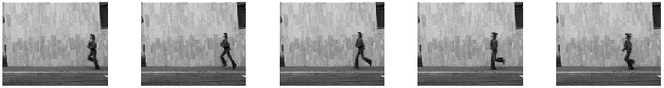
\includegraphics[width=.3\textwidth, keepaspectratio]{../../10_recurrent/doc/images/recurrent_3.png} & Futás \\
	Nevek felismerése & Tegnap Józsi letörölte a\par termelési adatbázist. & Tegnap
\textcolor{red}{Józsi} letörölte a\par termelési adatbázist. \\
\end{tabularx}
\end{frame}

\begin{frame}{Szavak reprezentálása 1-hot vektorokkal}
\begin{columns}
\begin{column}{.7\textwidth}
\renewcommand{\arraystretch}{3.}
\begin{tabularx}{\textwidth}{m{3cm}m{5cm}}
\textbf{Input:} & A kedvenc sportom a foci.\\
\textbf{Reprezentáció:} & $X = \left[ x_{1},\;x_{2},\;x_{3},\;x_{4},\;x_{5},\right]$\\
\textbf{Szókincs}: & $\left[ \underset{1}{a},\;\underset{2}{foci},\;\underset{3}{kedvenc},\;\underset{4}{sportom} \right]$\\
\textbf{Reprezentáció}: & $foci = \left[ 0, 1, 0, 0 \right]$\par
$sportom = \left[ 0, 0, 0, 1 \right]$
\end{tabularx}
\end{column}
\hspace{-1cm}
\begin{column}{.45\textwidth}
\textbf{Problémák}:
\begin{itemize}
	\item Ha van egy $10.000$ szóból álló szövegtörzs, minden szava egy $10.000$ elemű vektorként lesz reprezentálva, aminek csak egyetlen eleme $1$, a többi $0$. \textbf{Ez nem egy skálázható megoldás}.
	\item \textbf{Nincs kapcsolat a szavak között}. A szavak külön-külön vannak kezelve, hasonló jelentésű szavak reprezentációja nagyban eltérhet. 
\end{itemize}
\end{column}
\end{columns}
\end{frame}

\begin{frame}{Szavak reprezentálása beágyazóvektorokkal}
\begin{columns}
\begin{column}{.4\textwidth}
\begin{block}{Beágyazás}
Egy szó beágyazása \textbf{egy magas dimenziójú vektortérben való numerikus reprezentáció}. Ezek a vektorok tartalmazzák a szavak \textbf{struktúráját, szemantikáját, és szintaktikai szerkezetét}.\par\smallskip
Ezáltal képesek a mélytanuló modellek elsajátítani a szavak közötti hasonlóságokat és az egyes szavak jelentését. 
\end{block}
\end{column}
\begin{column}{.6\textwidth}
\begin{center}
\begin{tabular}{|c|c|c|c|c|c|}
\hline
& \textbf{Férfi} & \textbf{Nő} & \textbf{Király} & \textbf{Királynő} & \textbf{Alma} \\
\hline
\textbf{Nem} & $-1$ & $1$ & $-0.95$ & $0.97$ & $0.0$\\
\hline
\textbf{Előkelő} & $0.01$ & $0.02$ & $0.93$ & $0.95$ & $-0.01$\\
\hline
\textbf{Kor} & $0.03$ & $0.02$ & $0.7$ & $0.68$ & $0.03$\\
\hline
\textbf{Étel} & $0.04$ & $0.01$ & $0.02$ & $0.01$ & $0.96$\\
\hline
\end{tabular}
\end{center}
Tehát ebben az esetben például a férfi szó beágyazóvektora:
\begin{block}{}
\vspace{-0.2cm}
\[
e_{\textit{férfi}} = \left[ -1,\;0.01,\;0.03,\;0.04 \right]
\]
\end{block}
\end{column}
\end{columns}
\end{frame}

\begin{frame}{Beágyazóvektorok reprezentálása}
\begin{columns}
\begin{column}{.5\textwidth}
A beágyazóvektorok használatával lehetőség nyílik a szavak hasonlóságának kiszámítására.\par\smallskip
Az egymáshoz jelentés tartalmilag \textbf{közelebb álló szavak beágyazóvektorainak matematikai távolsága alacsonyabb lesz, mint az egymástól távolabb eső szavaké}.
\par\smallskip
Ezáltal továbbá lehetséges analógiák kiszámítása is. \emph{A férfi és a király olyanok egymásnak, mint a nő és a királynő.}
\end{column}
\begin{column}{.5\textwidth}
\begin{center}
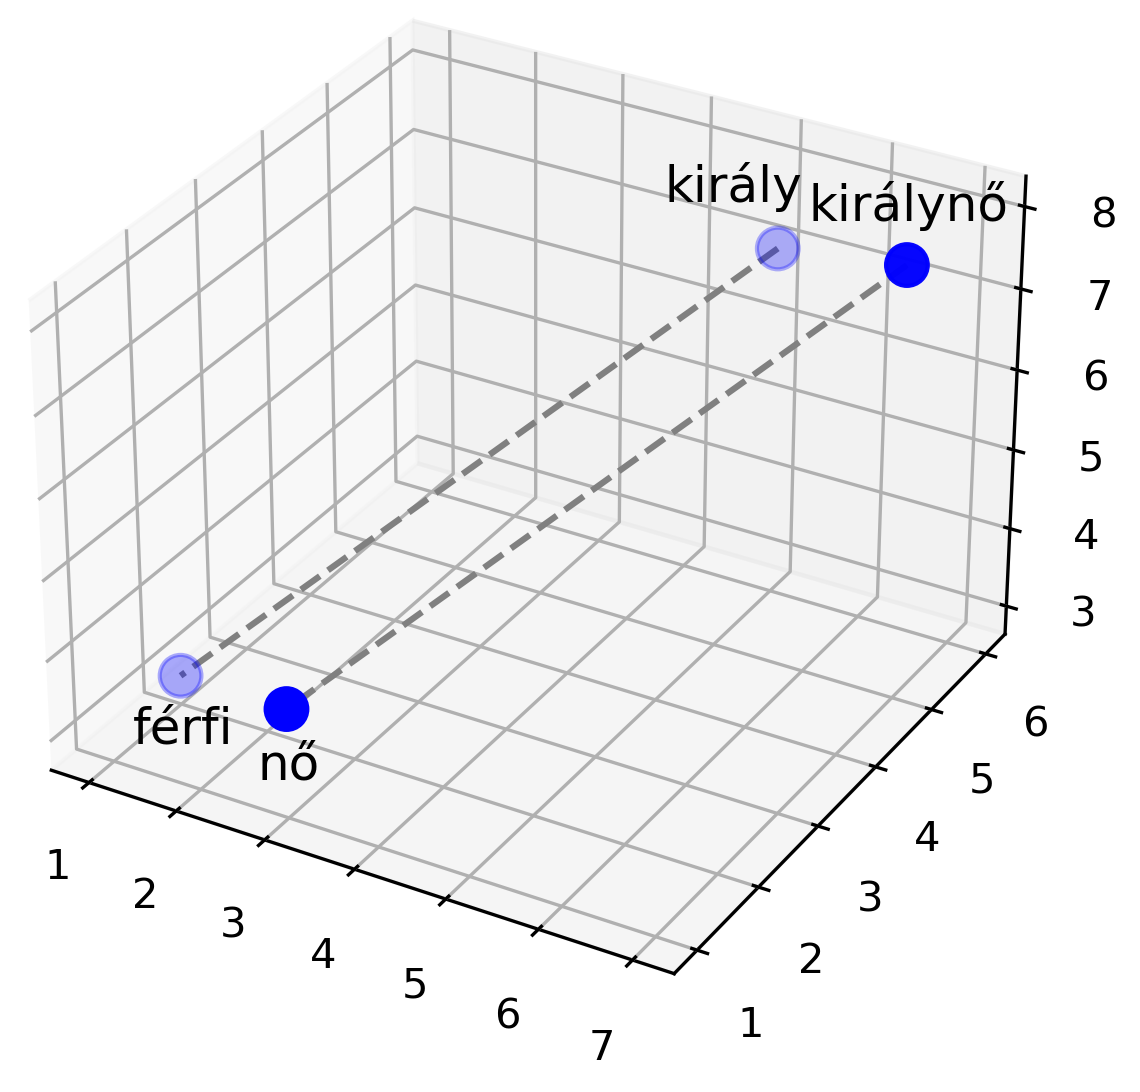
\includegraphics[width=7cm, height=7cm, keepaspectratio]{images/embedding_vectors_.png}
\end{center}
\end{column}
\end{columns}
\end{frame}

\begin{frame}{Beágyazások vizualizálása}
\begin{columns}
\begin{column}{.5\textwidth}
Dimenziócsökkentő algoritmusok segítségével lehetőség nyílik \textbf{a magasabb dimenziós vektorok alacsonyabb térben való reprezentációjára}. Az egyik ilyen algoritmus a T-SNE, ami jól használható komplex input adatok esetén.\par\smallskip
Ez hasznos a következő problémák esetén:
\begin{itemize}
	\item Vizualizáció
	\item Klaszterezés
	\item Adatminőség mérése
	\item Szemantikai kapcsolatok elemzése
	\item Hiperparaméter hangolás
\end{itemize}
\end{column}
\begin{column}{.5\textwidth}
\begin{center}
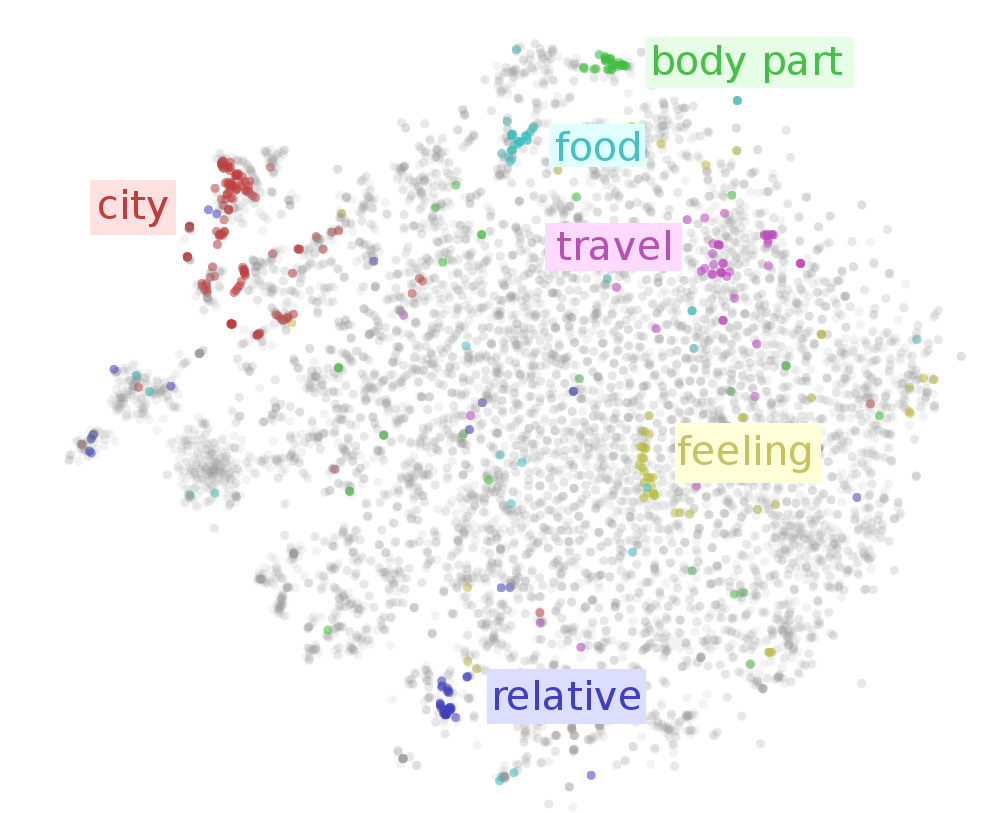
\includegraphics[width=7cm, height=7cm, keepaspectratio]{images/transformer_1.png}
\end{center}
\end{column}
\end{columns}
\end{frame}

\section{Transzformáló architektúrák}

\begin{frame}{}
\tableofcontents[currentsection]
\end{frame}

\begin{frame}{Hagyományos visszacsatolásos architektúrák}
\begin{columns}
\begin{column}{.5\textwidth}
A visszacsatolásos neurális hálózatok (RNN) olyan mesterséges neurális hálózatok, amelyek képesek kezelni \textbf{időbeli szekvenciákat és más időfüggő adatokat}.\par\smallskip
Ezek a hálózatok olyan struktúrával rendelkeznek, amely lehetővé teszi a \textbf{korábbi lépések eredményeinek visszacsatolását az aktuális lépésbe}. Ennek eredményeként képesek tartani az emlékezetüket korábbi állapotokról, és ezáltal kezelni a szekvenciális adatokat
\end{column}
\begin{column}{.5\textwidth}
\begin{center}
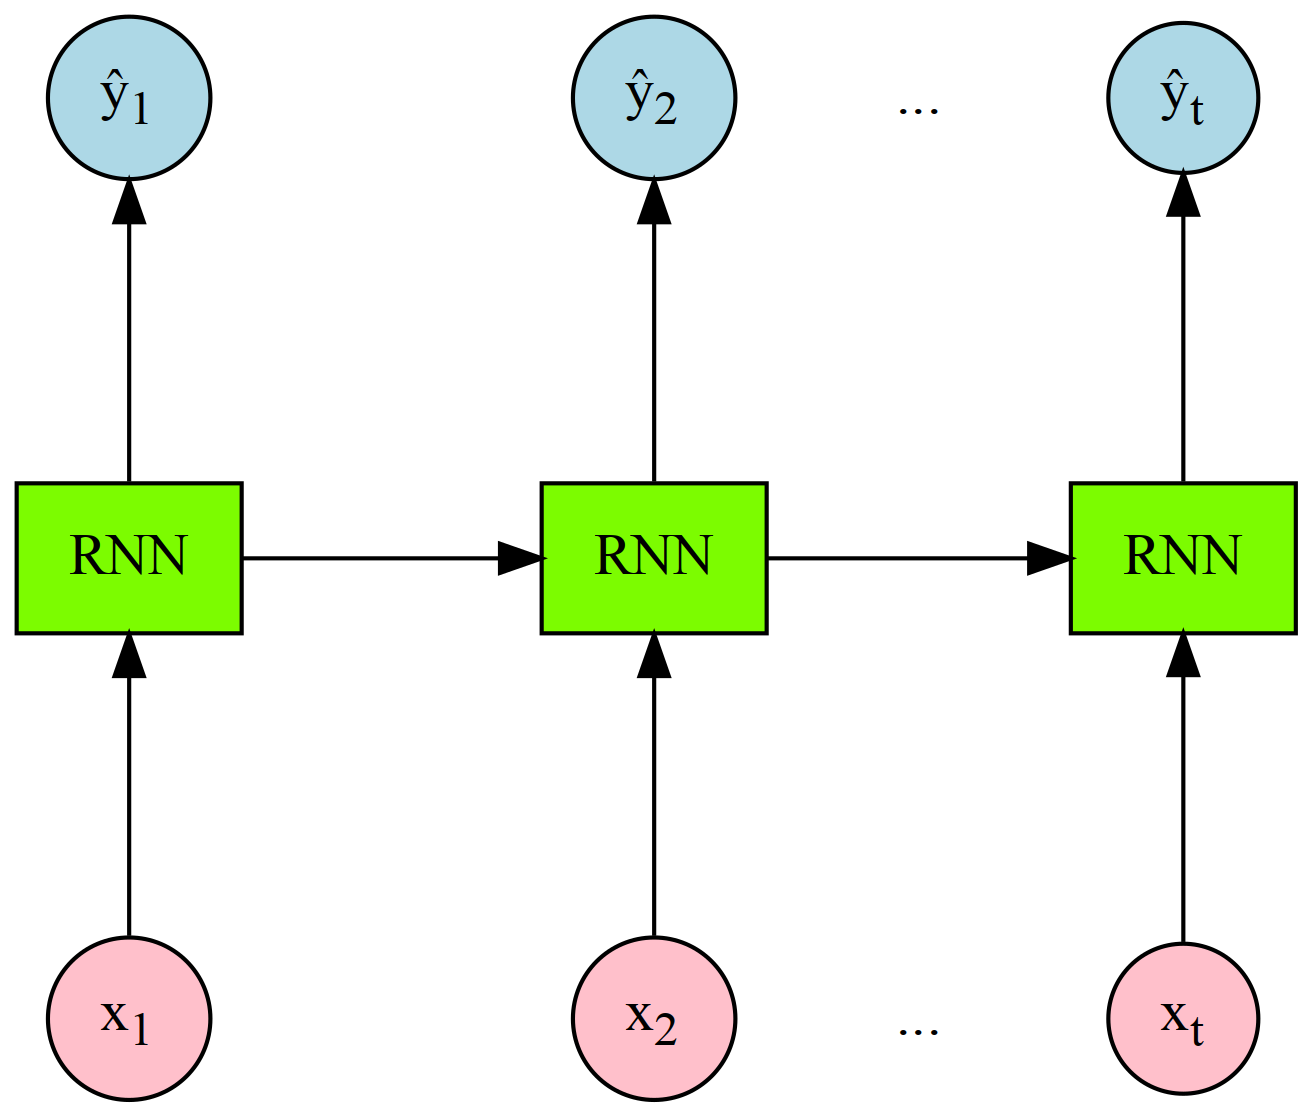
\includegraphics[height=5.5cm, width=\textwidth, keepaspectratio]{../../10_recurrent/doc/graphs/recurrent_4.png}
\end{center}
\end{column}
\end{columns}
\end{frame}

\begin{frame}{Önkódoló architektúrák}
Az önkódoló neurális hálózatok feladata az inputot átmásolni az outputba úgy, hogy közben megismeri az adatok alacsony szintű struktúráját:
\begin{columns}
\begin{column}{.5\textwidth}
\begin{itemize}
	\item \textbf{Kódoló}: A bemeneti adatokat tömöríti egy rövidebb, alacsony dimenziójú reprezentációba.
	\item \textbf{Látens tér}: Az az alacsony dimenziójú tér, amelyben a kódoló reprezentálja a bemeneti adatokat. Ez a tér tartalmazza az információkat a bemenetről kompakt formában.
	\item \textbf{Dekódoló}: Feladata a látens térben lévő reprezentációt visszaalakítani eredeti vagy közelítőleges formájára.
\end{itemize}
\end{column}
\begin{column}{.5\textwidth}
\begin{center}
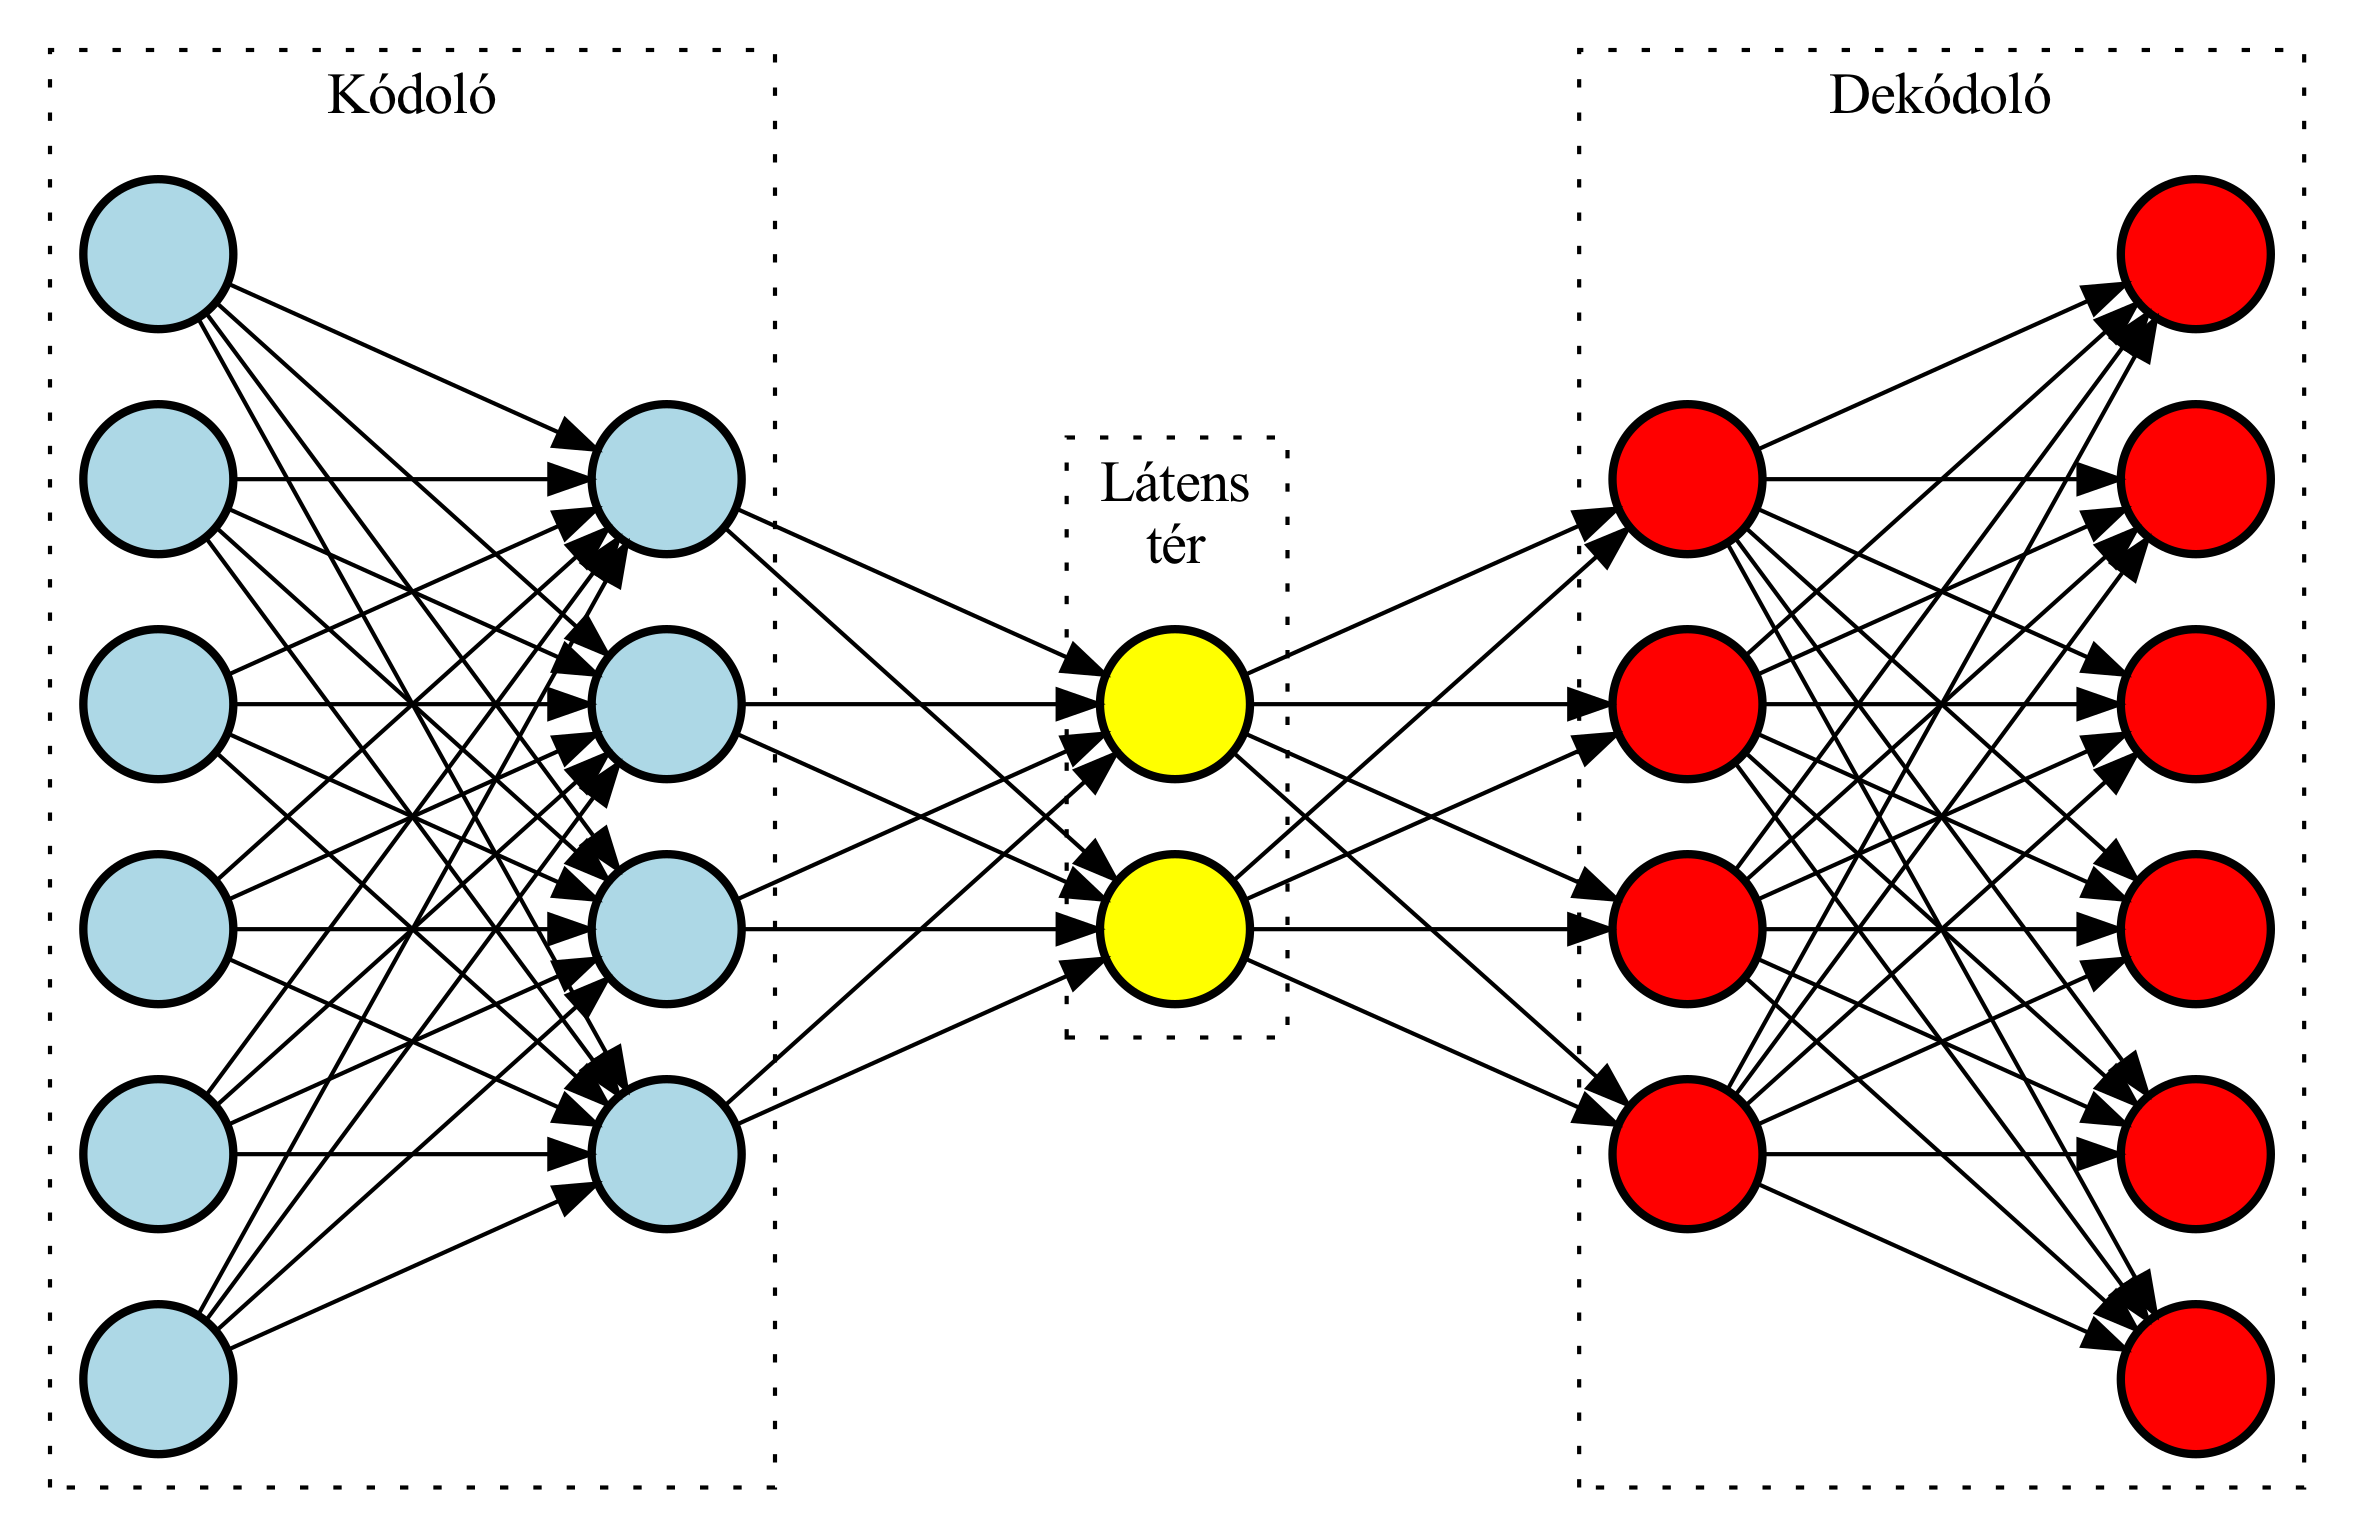
\includegraphics[height=7cm, width=7cm, keepaspectratio]{../../7_dl/doc/graphs/dl_4.png}
\end{center}
\end{column}
\end{columns}
\end{frame}

\begin{frame}{Transzformáló architektúrák}
A transzformáló architektúrák rendkívül sokoldalúak és hatékonyak a mesterséges mélytanulásban. A transzformálók feladata \textbf{két szekvencia közötti leképezés megtanulása}. Rendkívül jól teljesítenek olyan területeken mint a \textbf{természetes nyelvfeldolgozás, képfelismerés, hangfeldolgozás, megerősítéses tanulás}.
\begin{center}
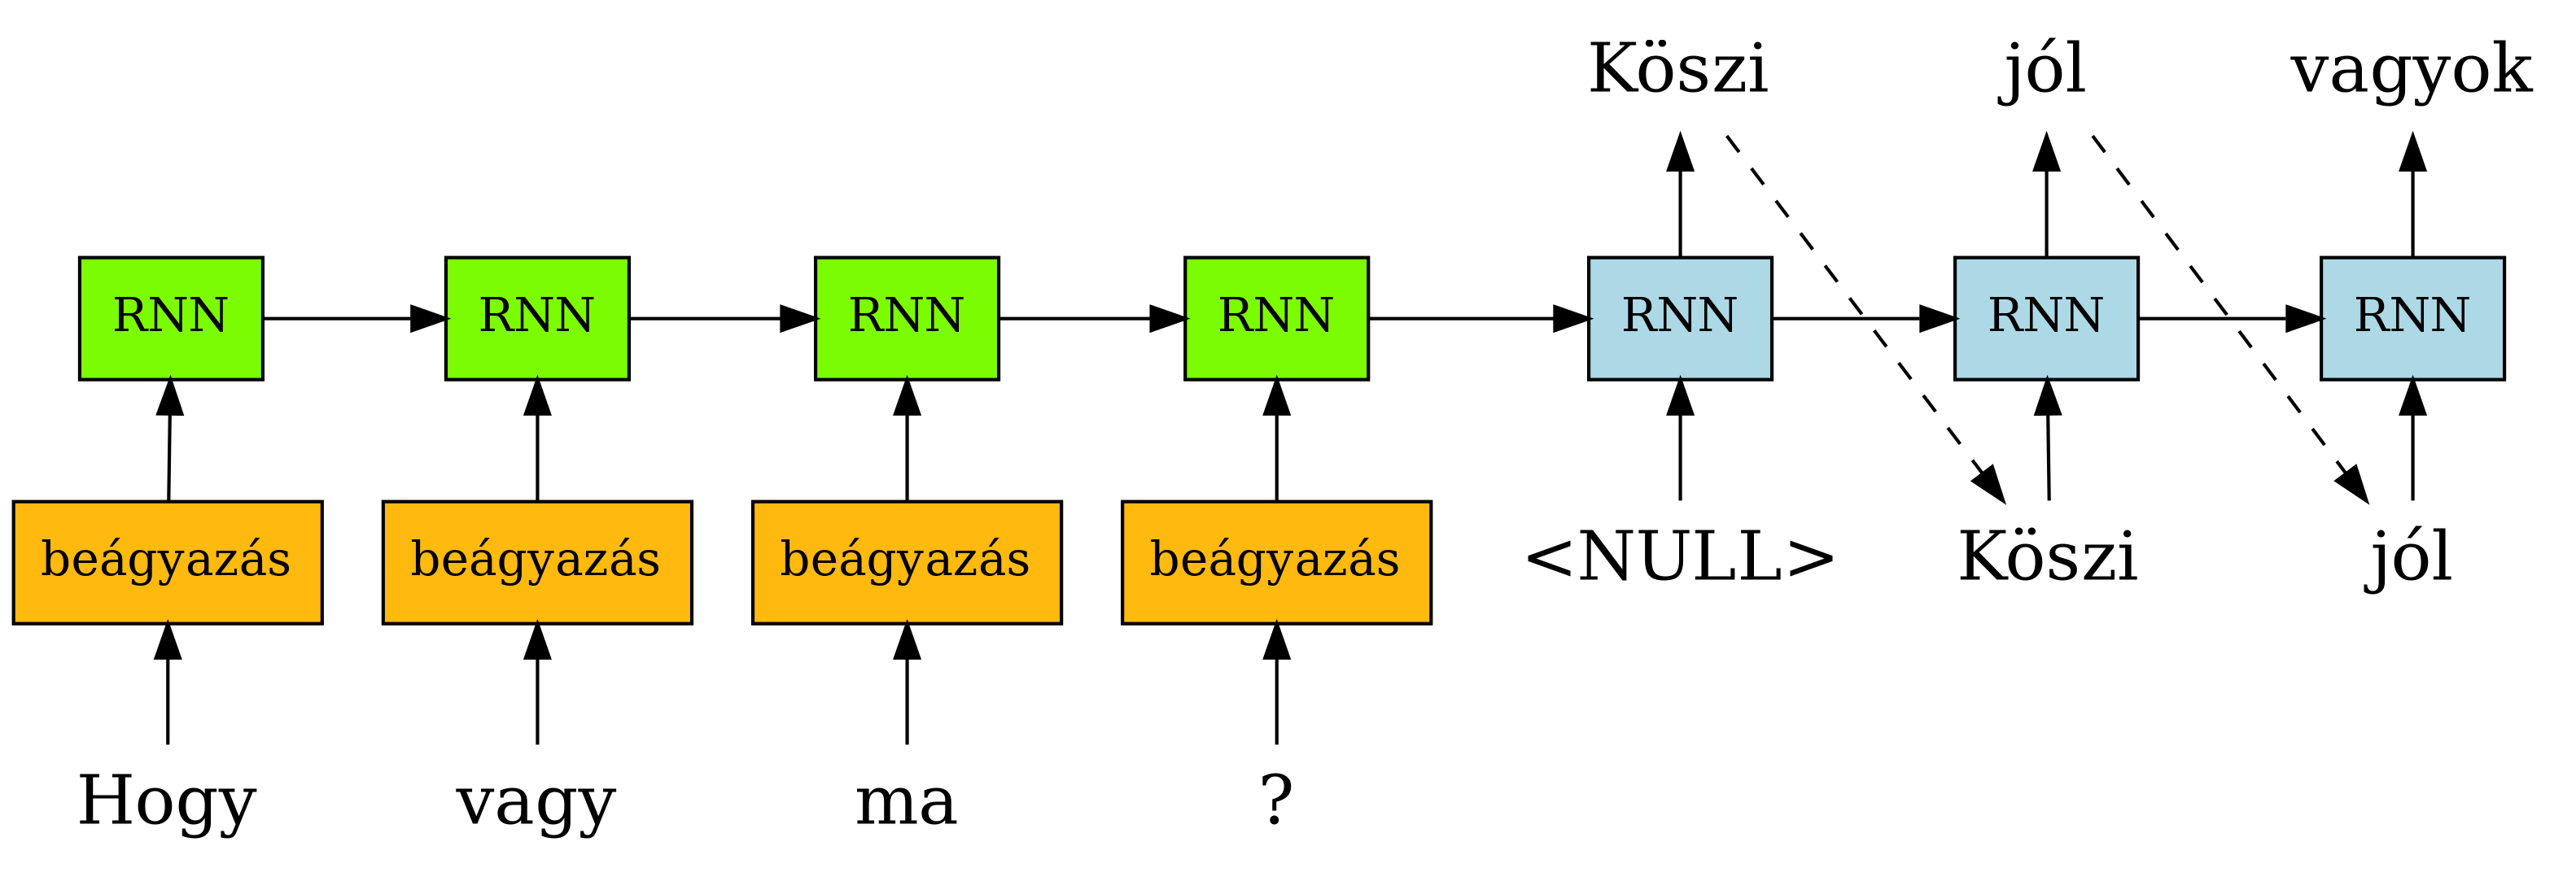
\includegraphics[width=14cm, height=7cm, keepaspectratio]{graphs/transformer_1.png}
\end{center}
\end{frame}

\begin{frame}{Gépi fordítás}
A transzformáló architektúrák \textbf{jól képesek teljesíteni a gépi fordítás területén}. Hasonlóan az önkódoló architektúrákhoz a fő részei a \textbf{kódoló} az input feldolgozására, a \textbf{látens} tér az input reprezentálására és a \textbf{dekódoló} az output előállítására. 
\begin{center}
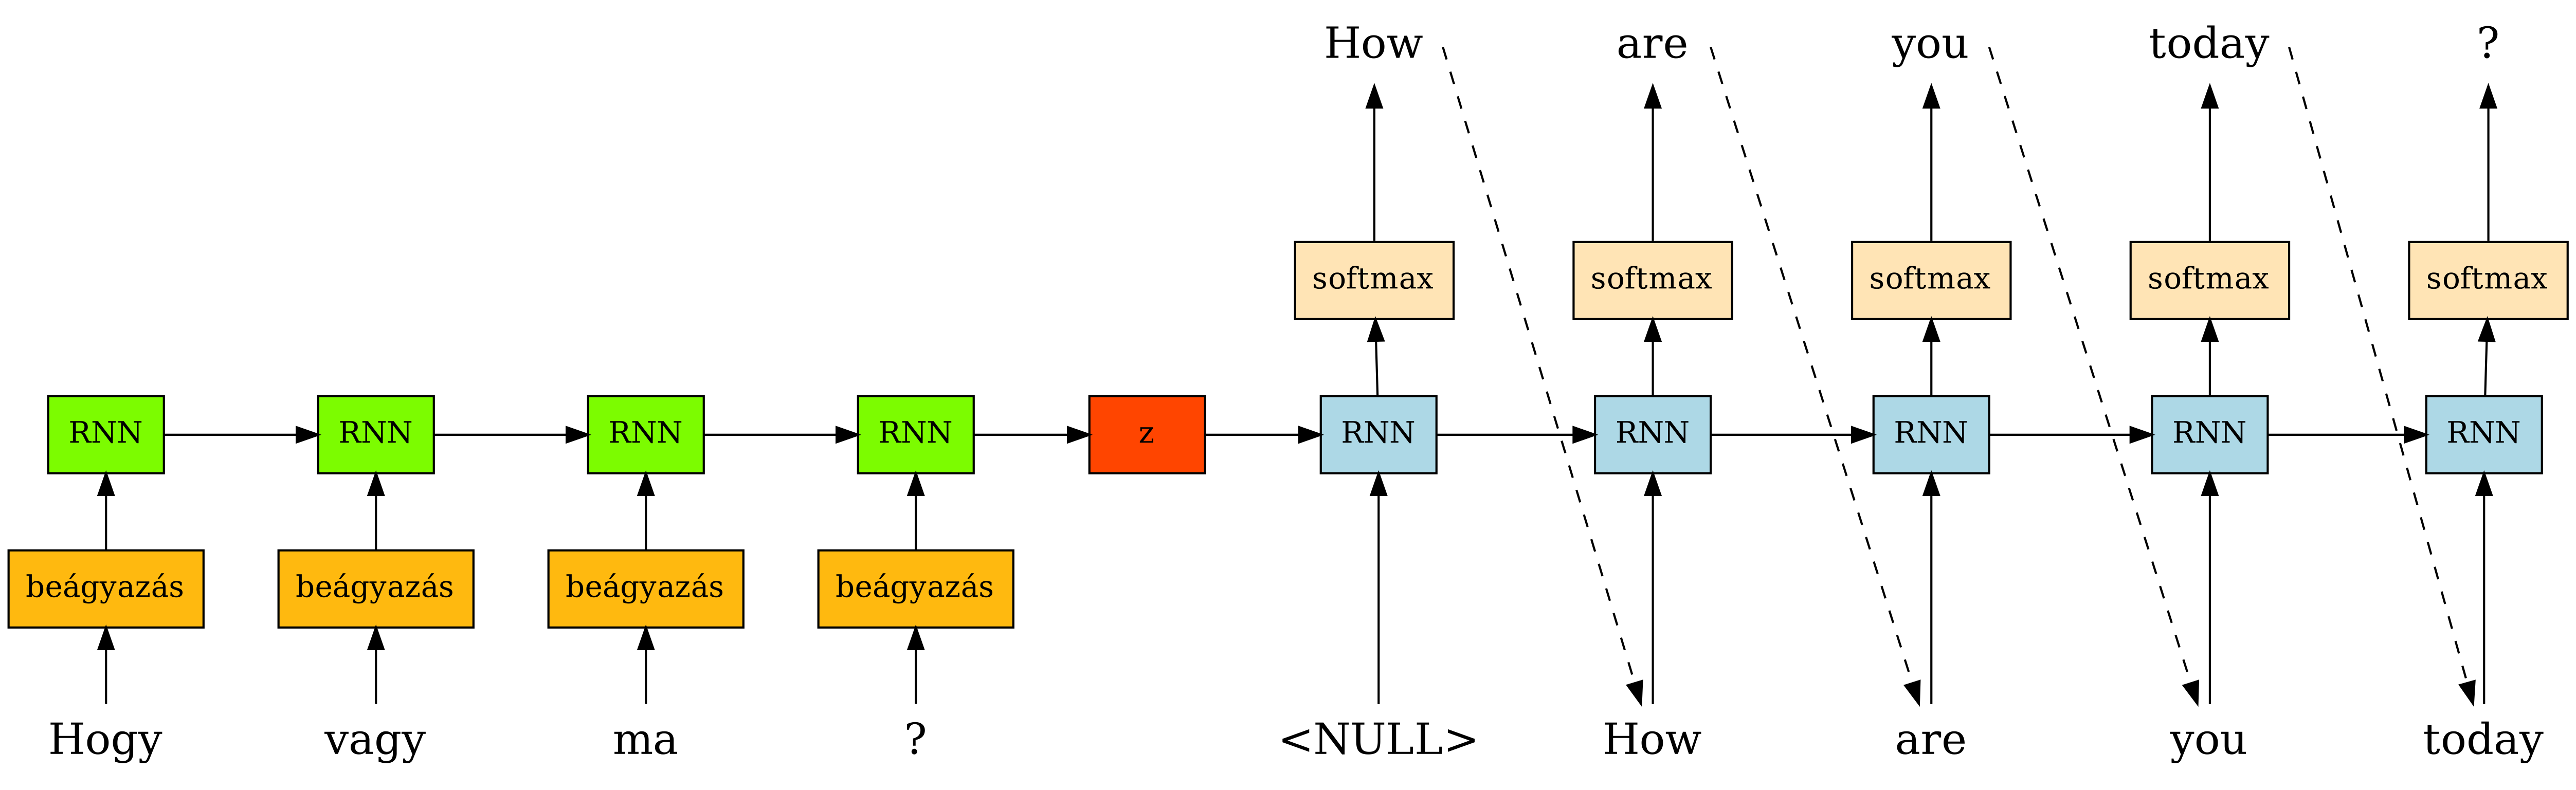
\includegraphics[width=14cm, height=7cm, keepaspectratio]{graphs/transformer_2.png}
\end{center}
\end{frame}

\begin{frame}{Kódoló}
A transzformáló architektúrákban a kódoló feladata az input adatok feldolgozása és egy \textbf{értelmes, kontextusban gazdag reprezentáció létrehozása}. Az kódolónak alapvető szerepe van az input sorozat megértésében és az alatta rejlő információk megragadásában. Az általa feldolgozott információ a $z$ kontextus vektorban kerül átadásra a dekódolónak, ami megfelel az utolsó cella rejtett állapotának.\par\medskip
\begin{center}
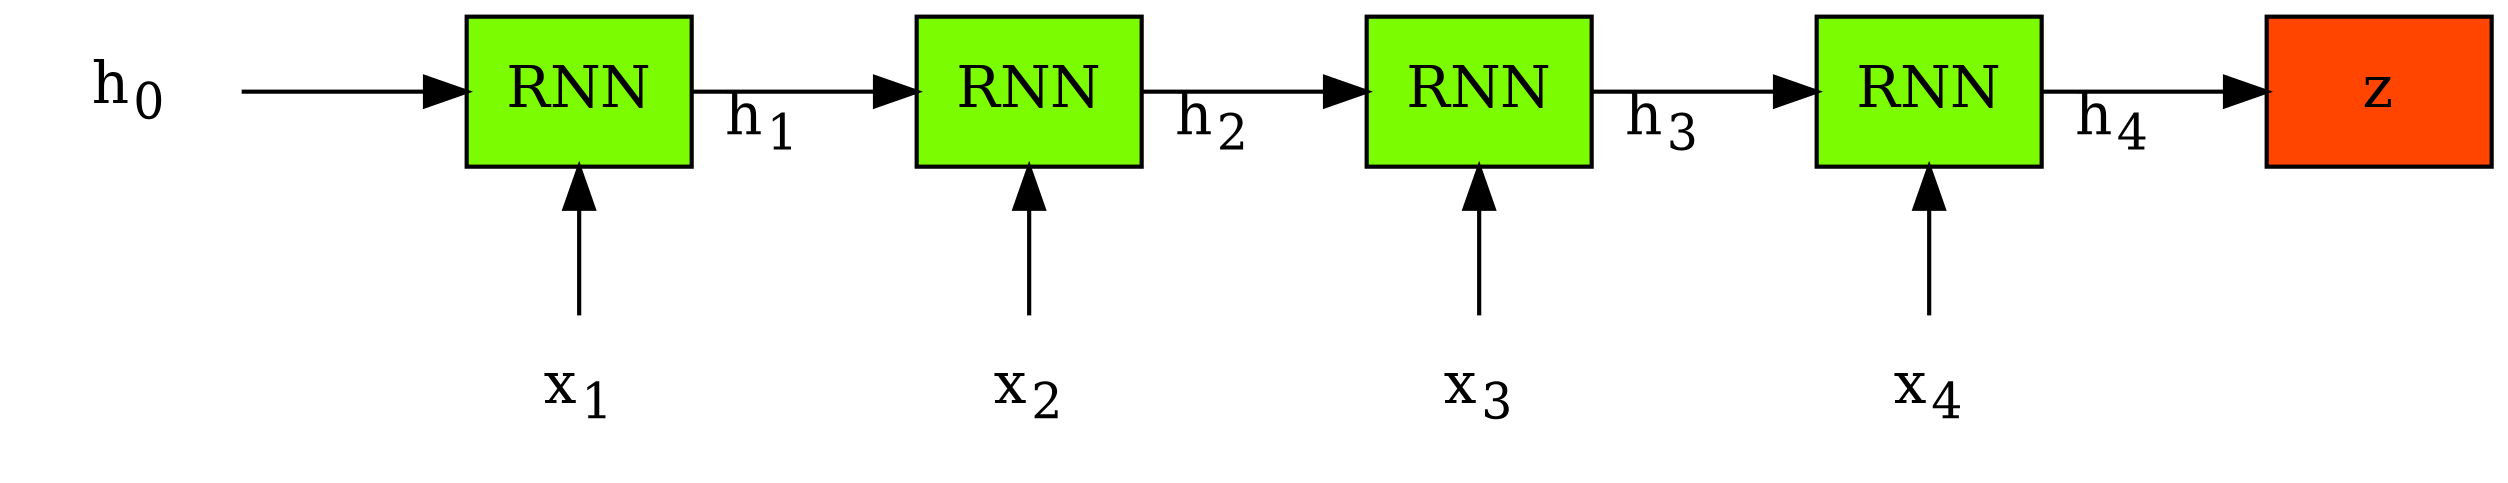
\includegraphics[width=14cm, keepaspectratio]{graphs/transformer_3.png}
\end{center}
\end{frame}

\begin{frame}{Dekódoló}
A dekódoló feladata a transzformáló architektúrákban \textbf{az output sorozat létrehozása az input sorozat kontextualizált reprezentációjának felhasználásával}. Dekódolás a legelső cella null inputot kap, és utána minden cella az előző cella outputját kapja meg inputként: $x_0 = null,\; x_i = y_i,\; i>0$. 
\begin{center}
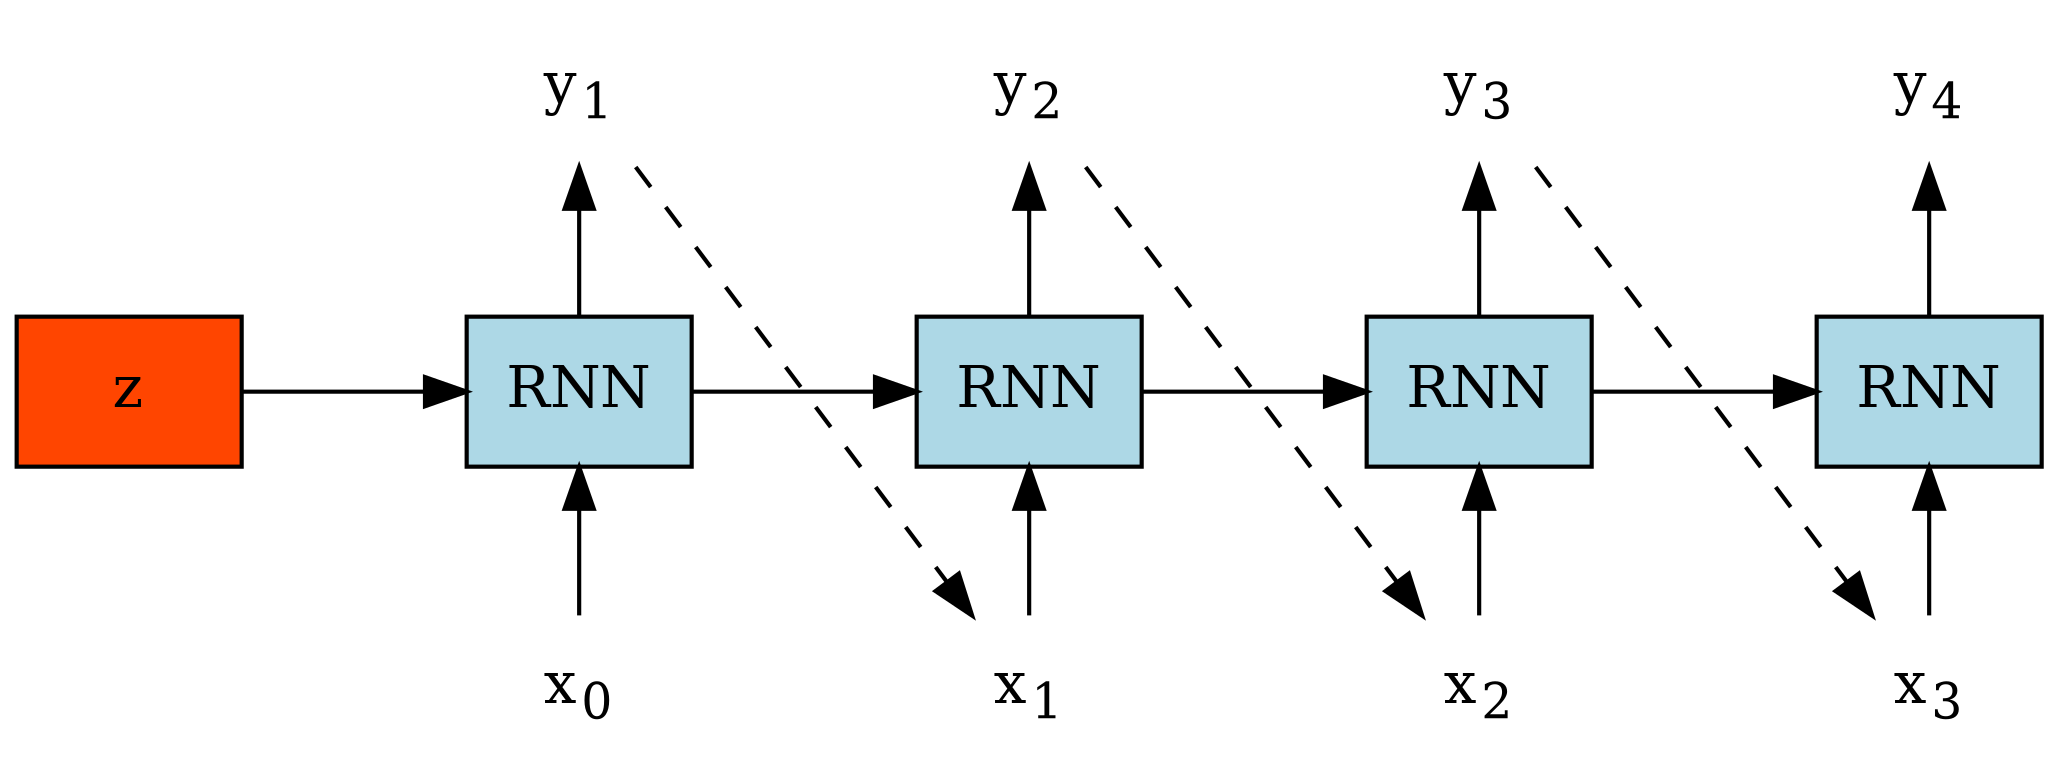
\includegraphics[width=14cm, height=7cm, keepaspectratio]{graphs/transformer_4.png}
\end{center}
\end{frame}

\begin{frame}{A transzformálók problémája}
Ha hosszú szekvenciákat kell generálniuk, a transzformálók gradiensei nagyon alacsonyak lesznek hiba visszaáramoltatás közben. Ez az \textbf{eltűnő gradiensek problémája}, és ahhoz vezet, hogy a hálózat elfelejti a korábbi információkat.\par\smallskip
Továbbá a modellnek \textbf{minden fontos információt egyetlen kontextus vektorba kell besűrítenie}. Ezzel a $z$ vektor lesz a tanulás szűk keresztmetszete. 
\begin{center}
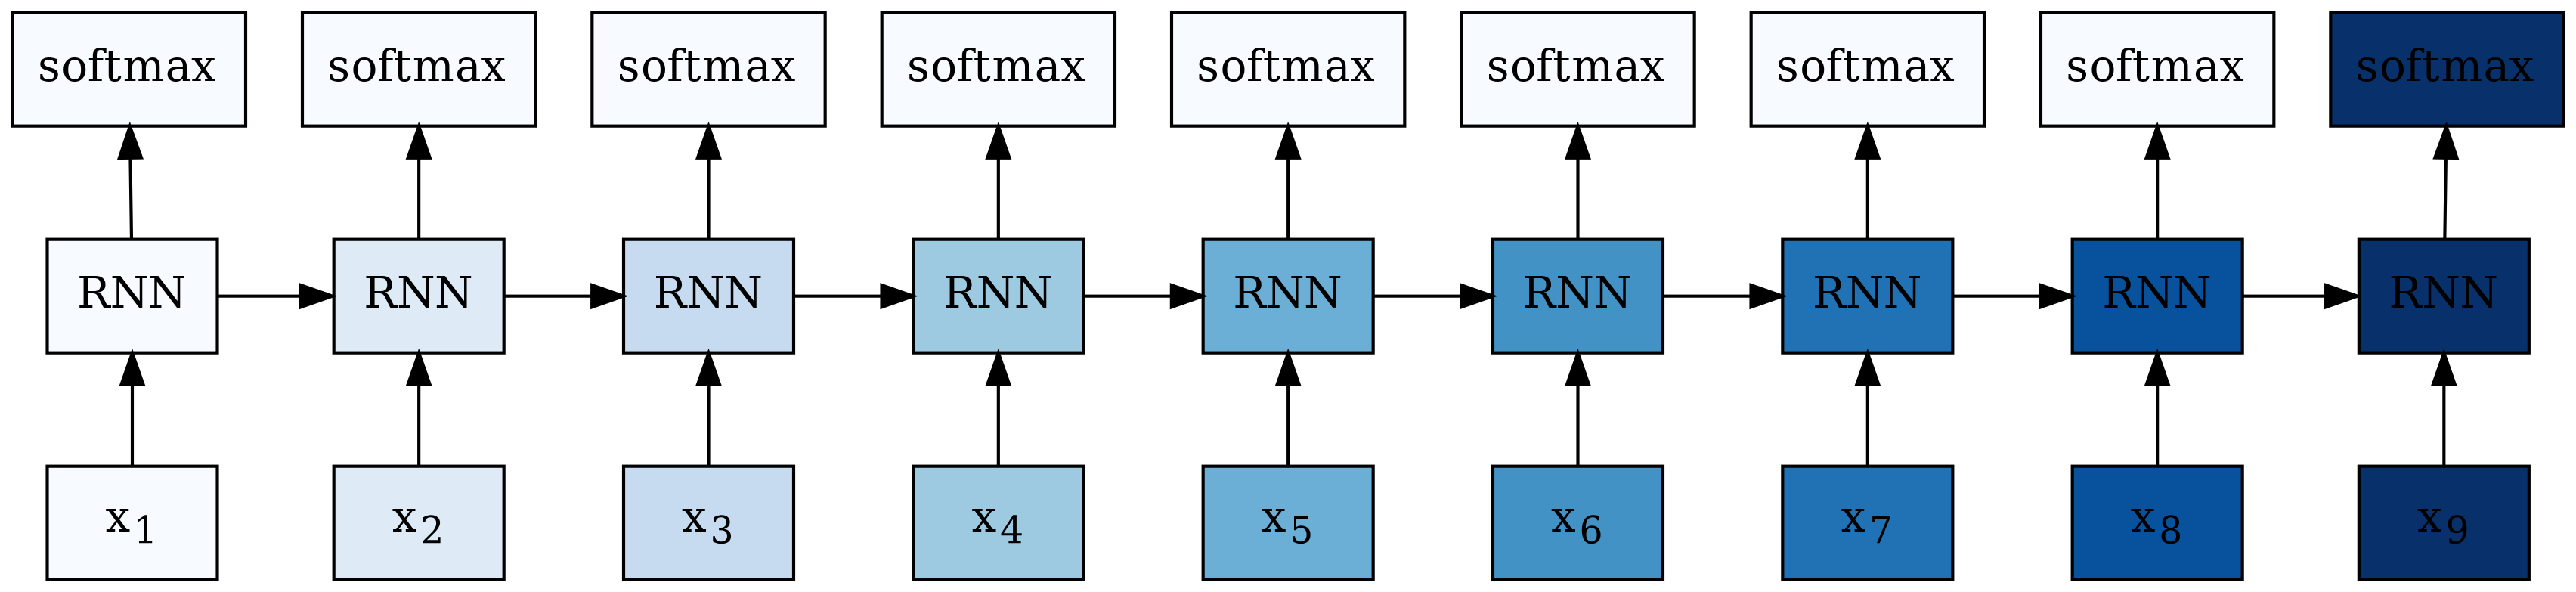
\includegraphics[width=14cm, height=7cm, keepaspectratio]{graphs/transformer_5.png}
\end{center}
\end{frame}

\section{Figyelmi mechanizmus}

\begin{frame}{}
\tableofcontents[currentsection]
\end{frame}

\begin{frame}{Figyelem alapjai}
\begin{columns}
\begin{column}{.5\textwidth}
\only<1>{Az alapvető megfontolás, hogy a $z$ kontextusvektornak legyen \textbf{közvetlen kapcsolata nem csak az input szekvencia utolsó eleméhez, hanem mindegyikhez}.\par\smallskip
Ezáltal a modellnek minden időlépésben minden vektor elemhez lesz hozzáférése, így lehetséges lesz megtanítani arra, \textbf{melyik állapot esetén melyik input elemre kell figyelmet fordítania}.}
\only<2>{A dekódoló hálózat figyelem értéke $i$ időlépésben:
\begin{block}{}
\vspace{-0.2cm}
\[ 
e_i=f(y_{i-1}, h_i) \in \mathbb{R}^n 
\]
\end{block}
A figyelmi értékek valószínűséggé alakítva és normalizálva:
\begin{block}{}
\[ 
\alpha_{ij} = \frac{e_{ij}}{\sum_{k=1}^{T_x}e_{ik}} 
\]
\end{block}
Ezáltal kontextus vektor $i$ időlépésben:
\begin{block}{}
\[
z_i = \sum_{j=1}^T \alpha_{ij}h_j
\]
\end{block}}
\end{column}
\begin{column}{.5\textwidth}
\begin{center}
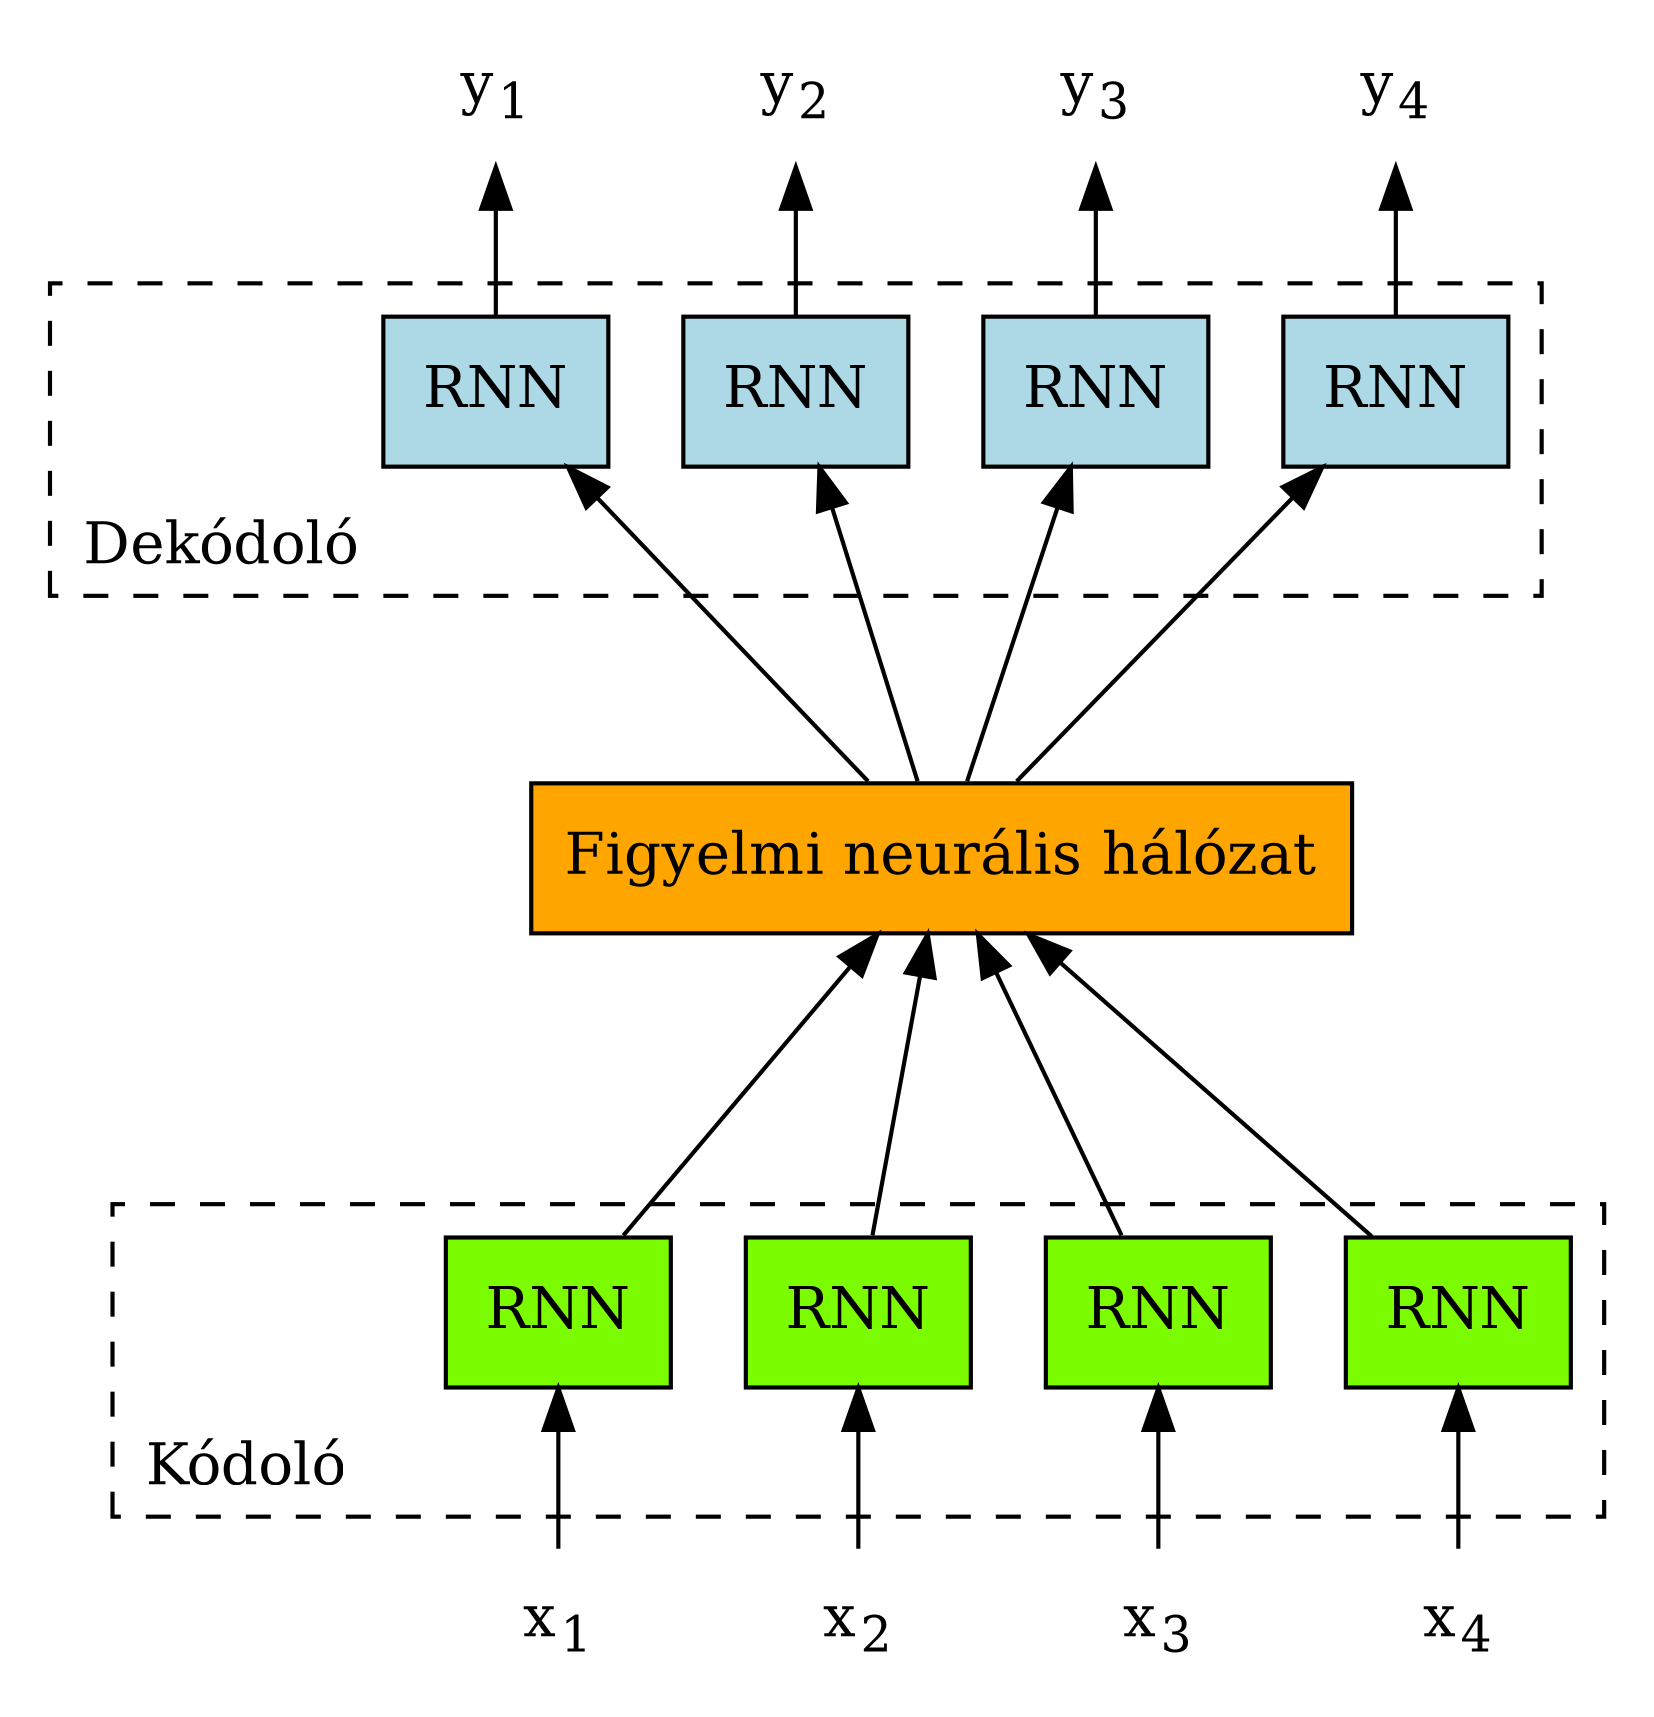
\includegraphics[width=7cm, height=7cm, keepaspectratio]{graphs/transformer_6.png}
\end{center}
\end{column}
\end{columns}
\end{frame}

\begin{frame}{Figyelmi modell}
\begin{columns}
\begin{column}{.3\textwidth}
\begin{block}{}
\vspace{-0.6cm}
\[ 
e_i=f(y_{i-1}, h_i) \in \mathbb{R}^n 
\]
\end{block}
\begin{block}{}
\[ 
\alpha_{ij} = \frac{e_{ij}}{\sum_{k=1}^{T_x}e_{ik}} 
\]
\end{block}
\begin{block}{}
\[
z_i = \sum_{j=1}^T \alpha_{ij}h_j
\]
\end{block}
\end{column}
\begin{column}{.7\textwidth}
\only<1>{\begin{center}
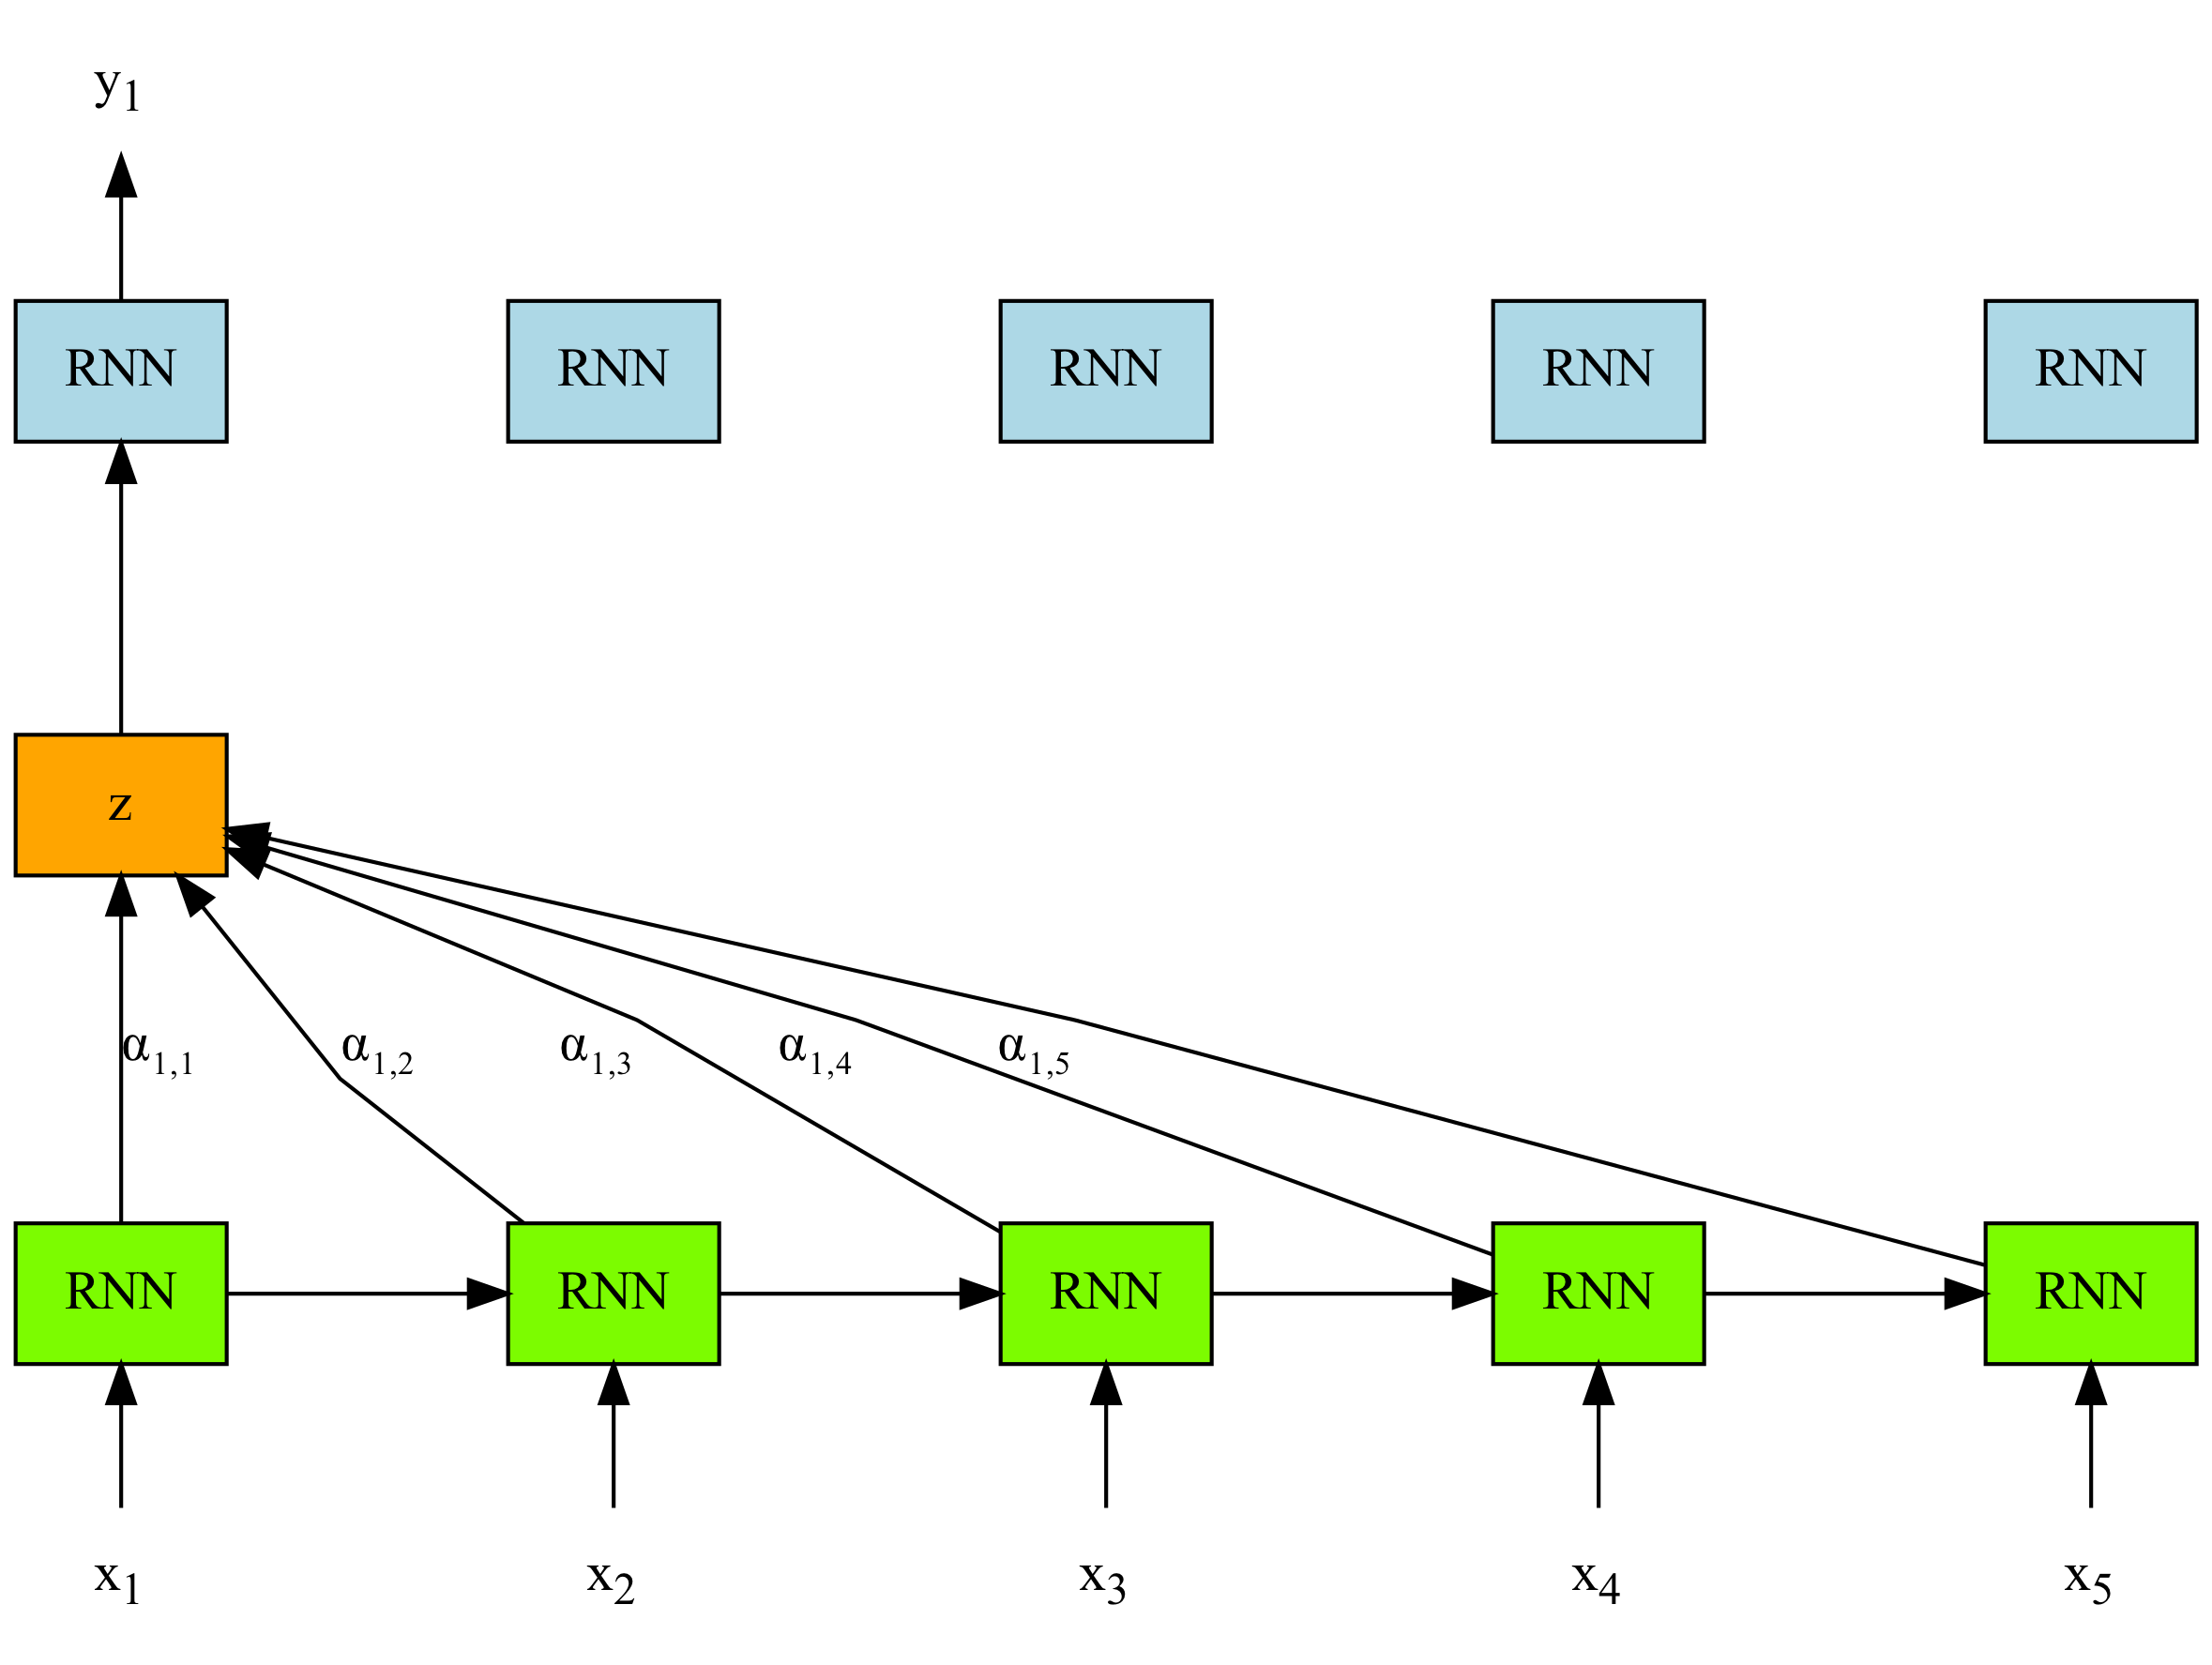
\includegraphics[width=14cm, height=7cm, keepaspectratio]{graphs/transformer_7.png}
\end{center}}
\only<2>{\begin{center}
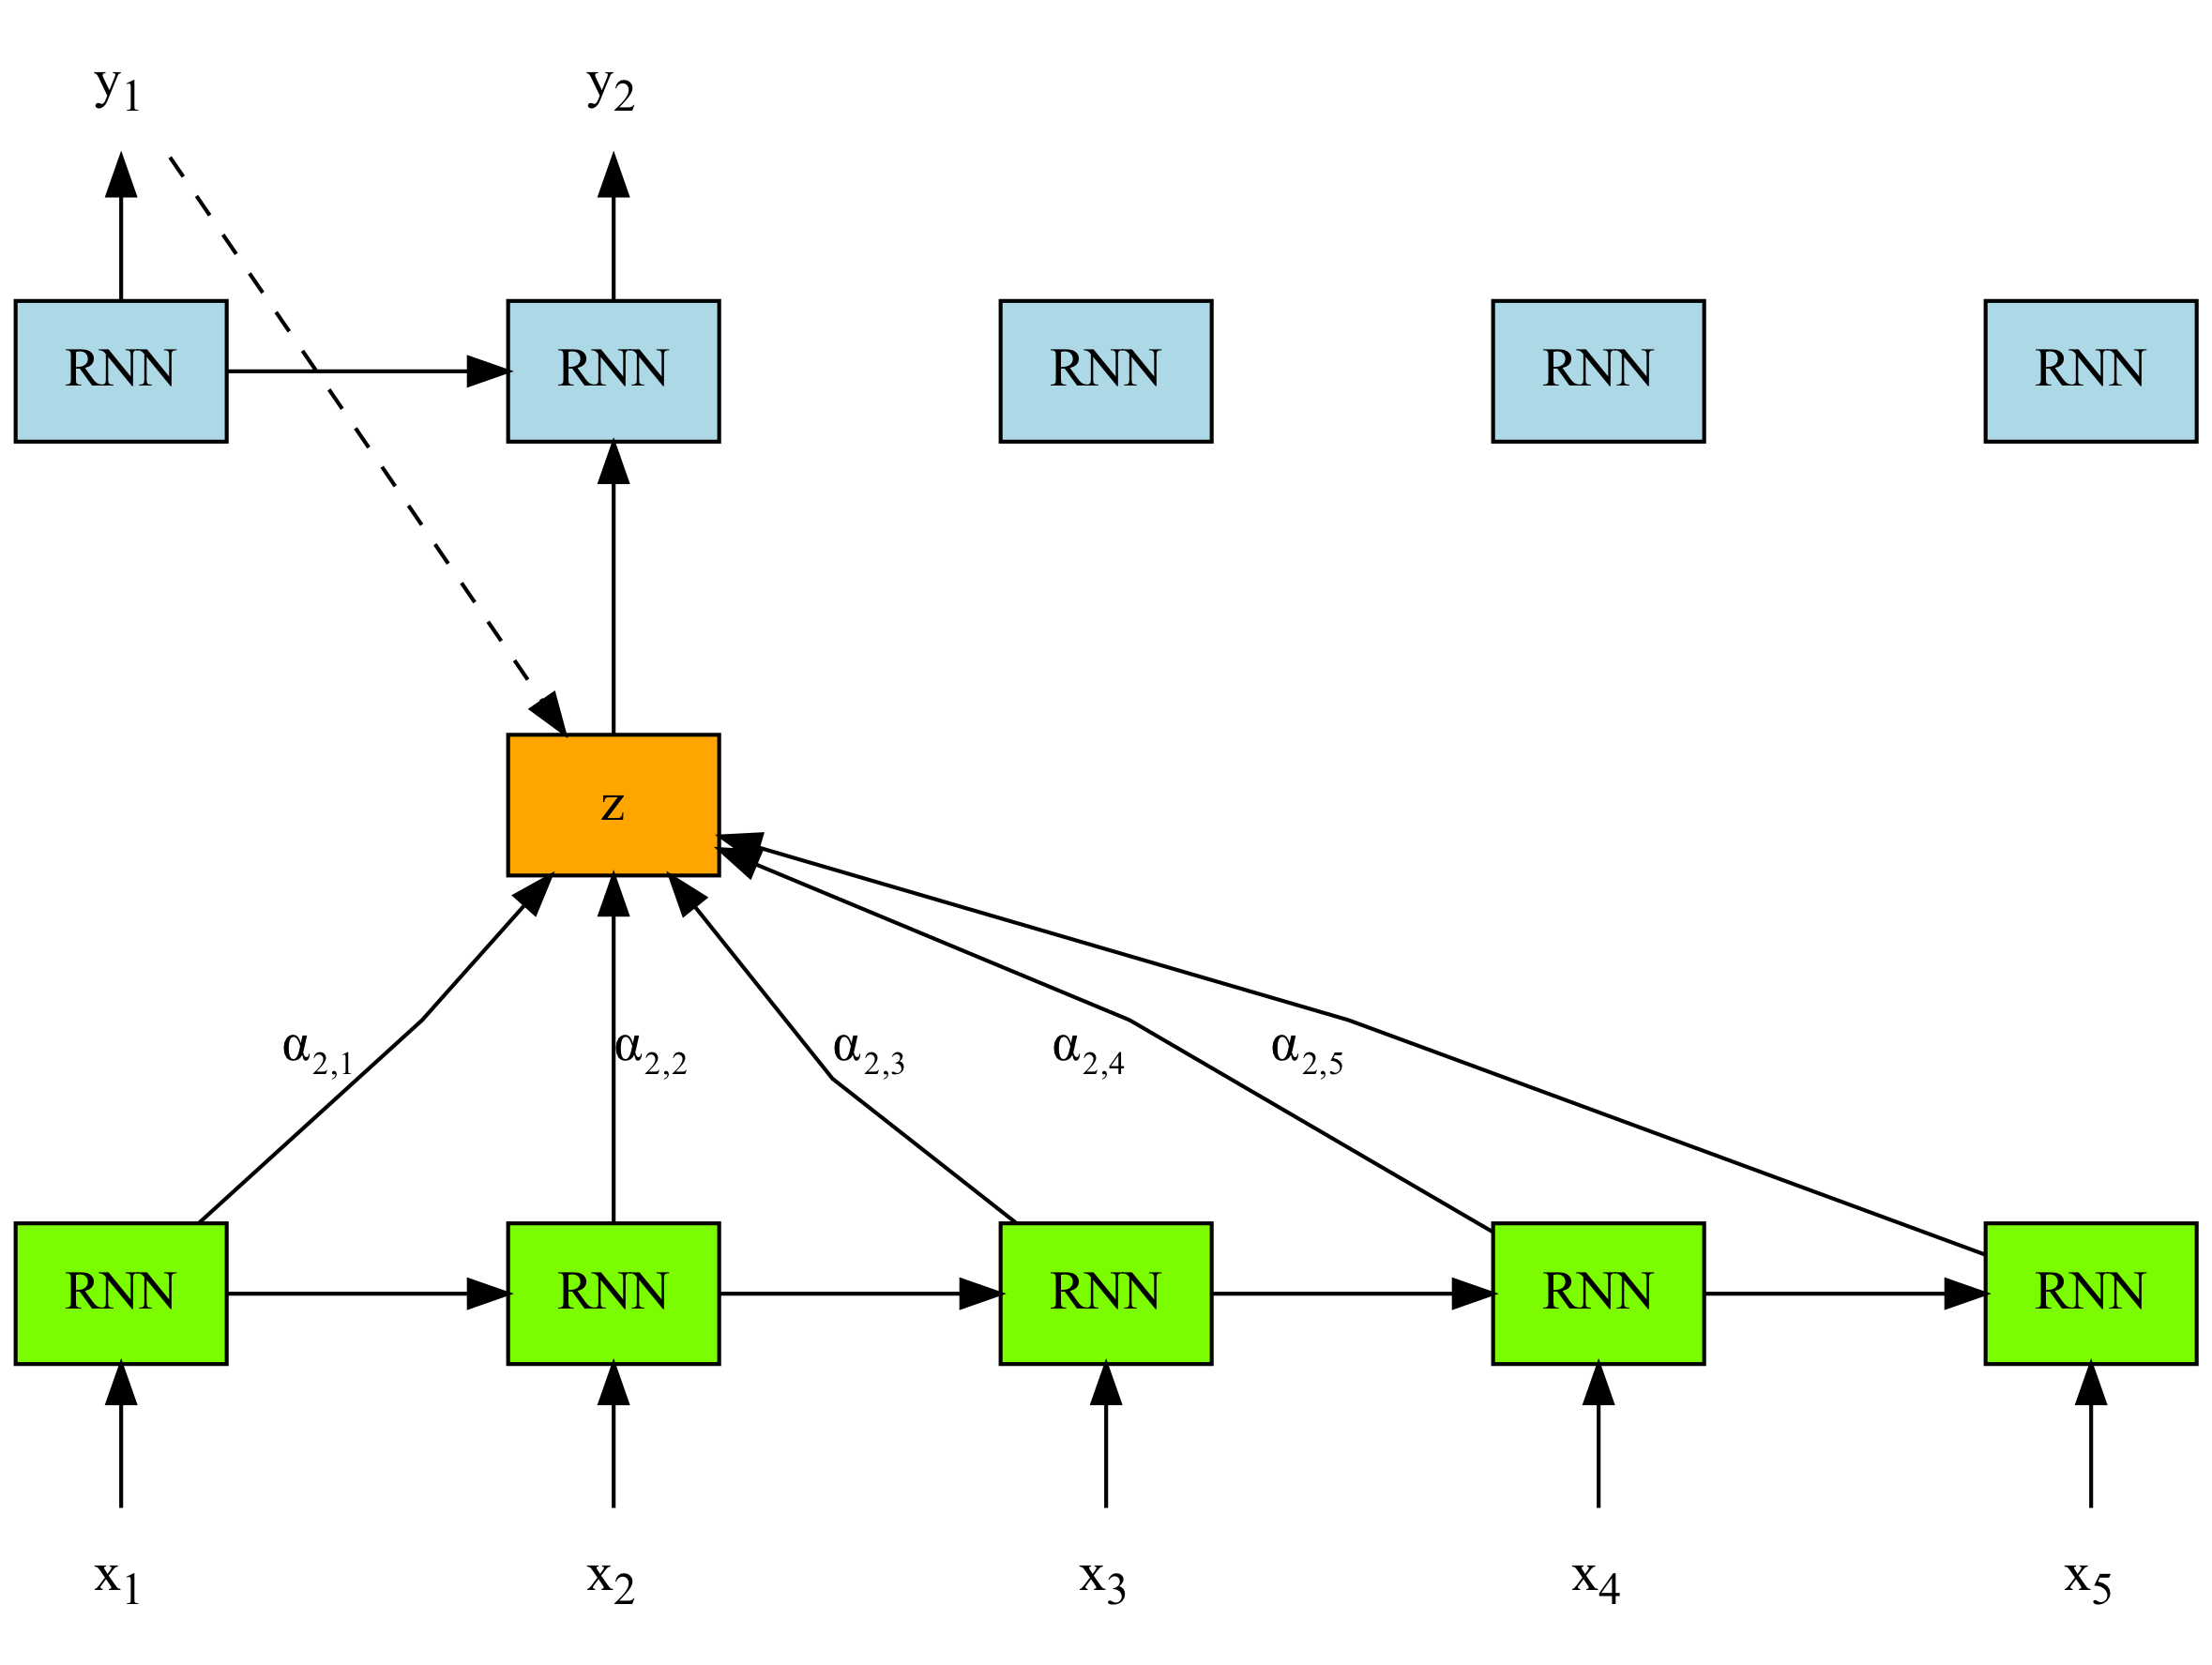
\includegraphics[width=14cm, height=7cm, keepaspectratio]{graphs/transformer_8.png}
\end{center}}
\only<3>{\begin{center}
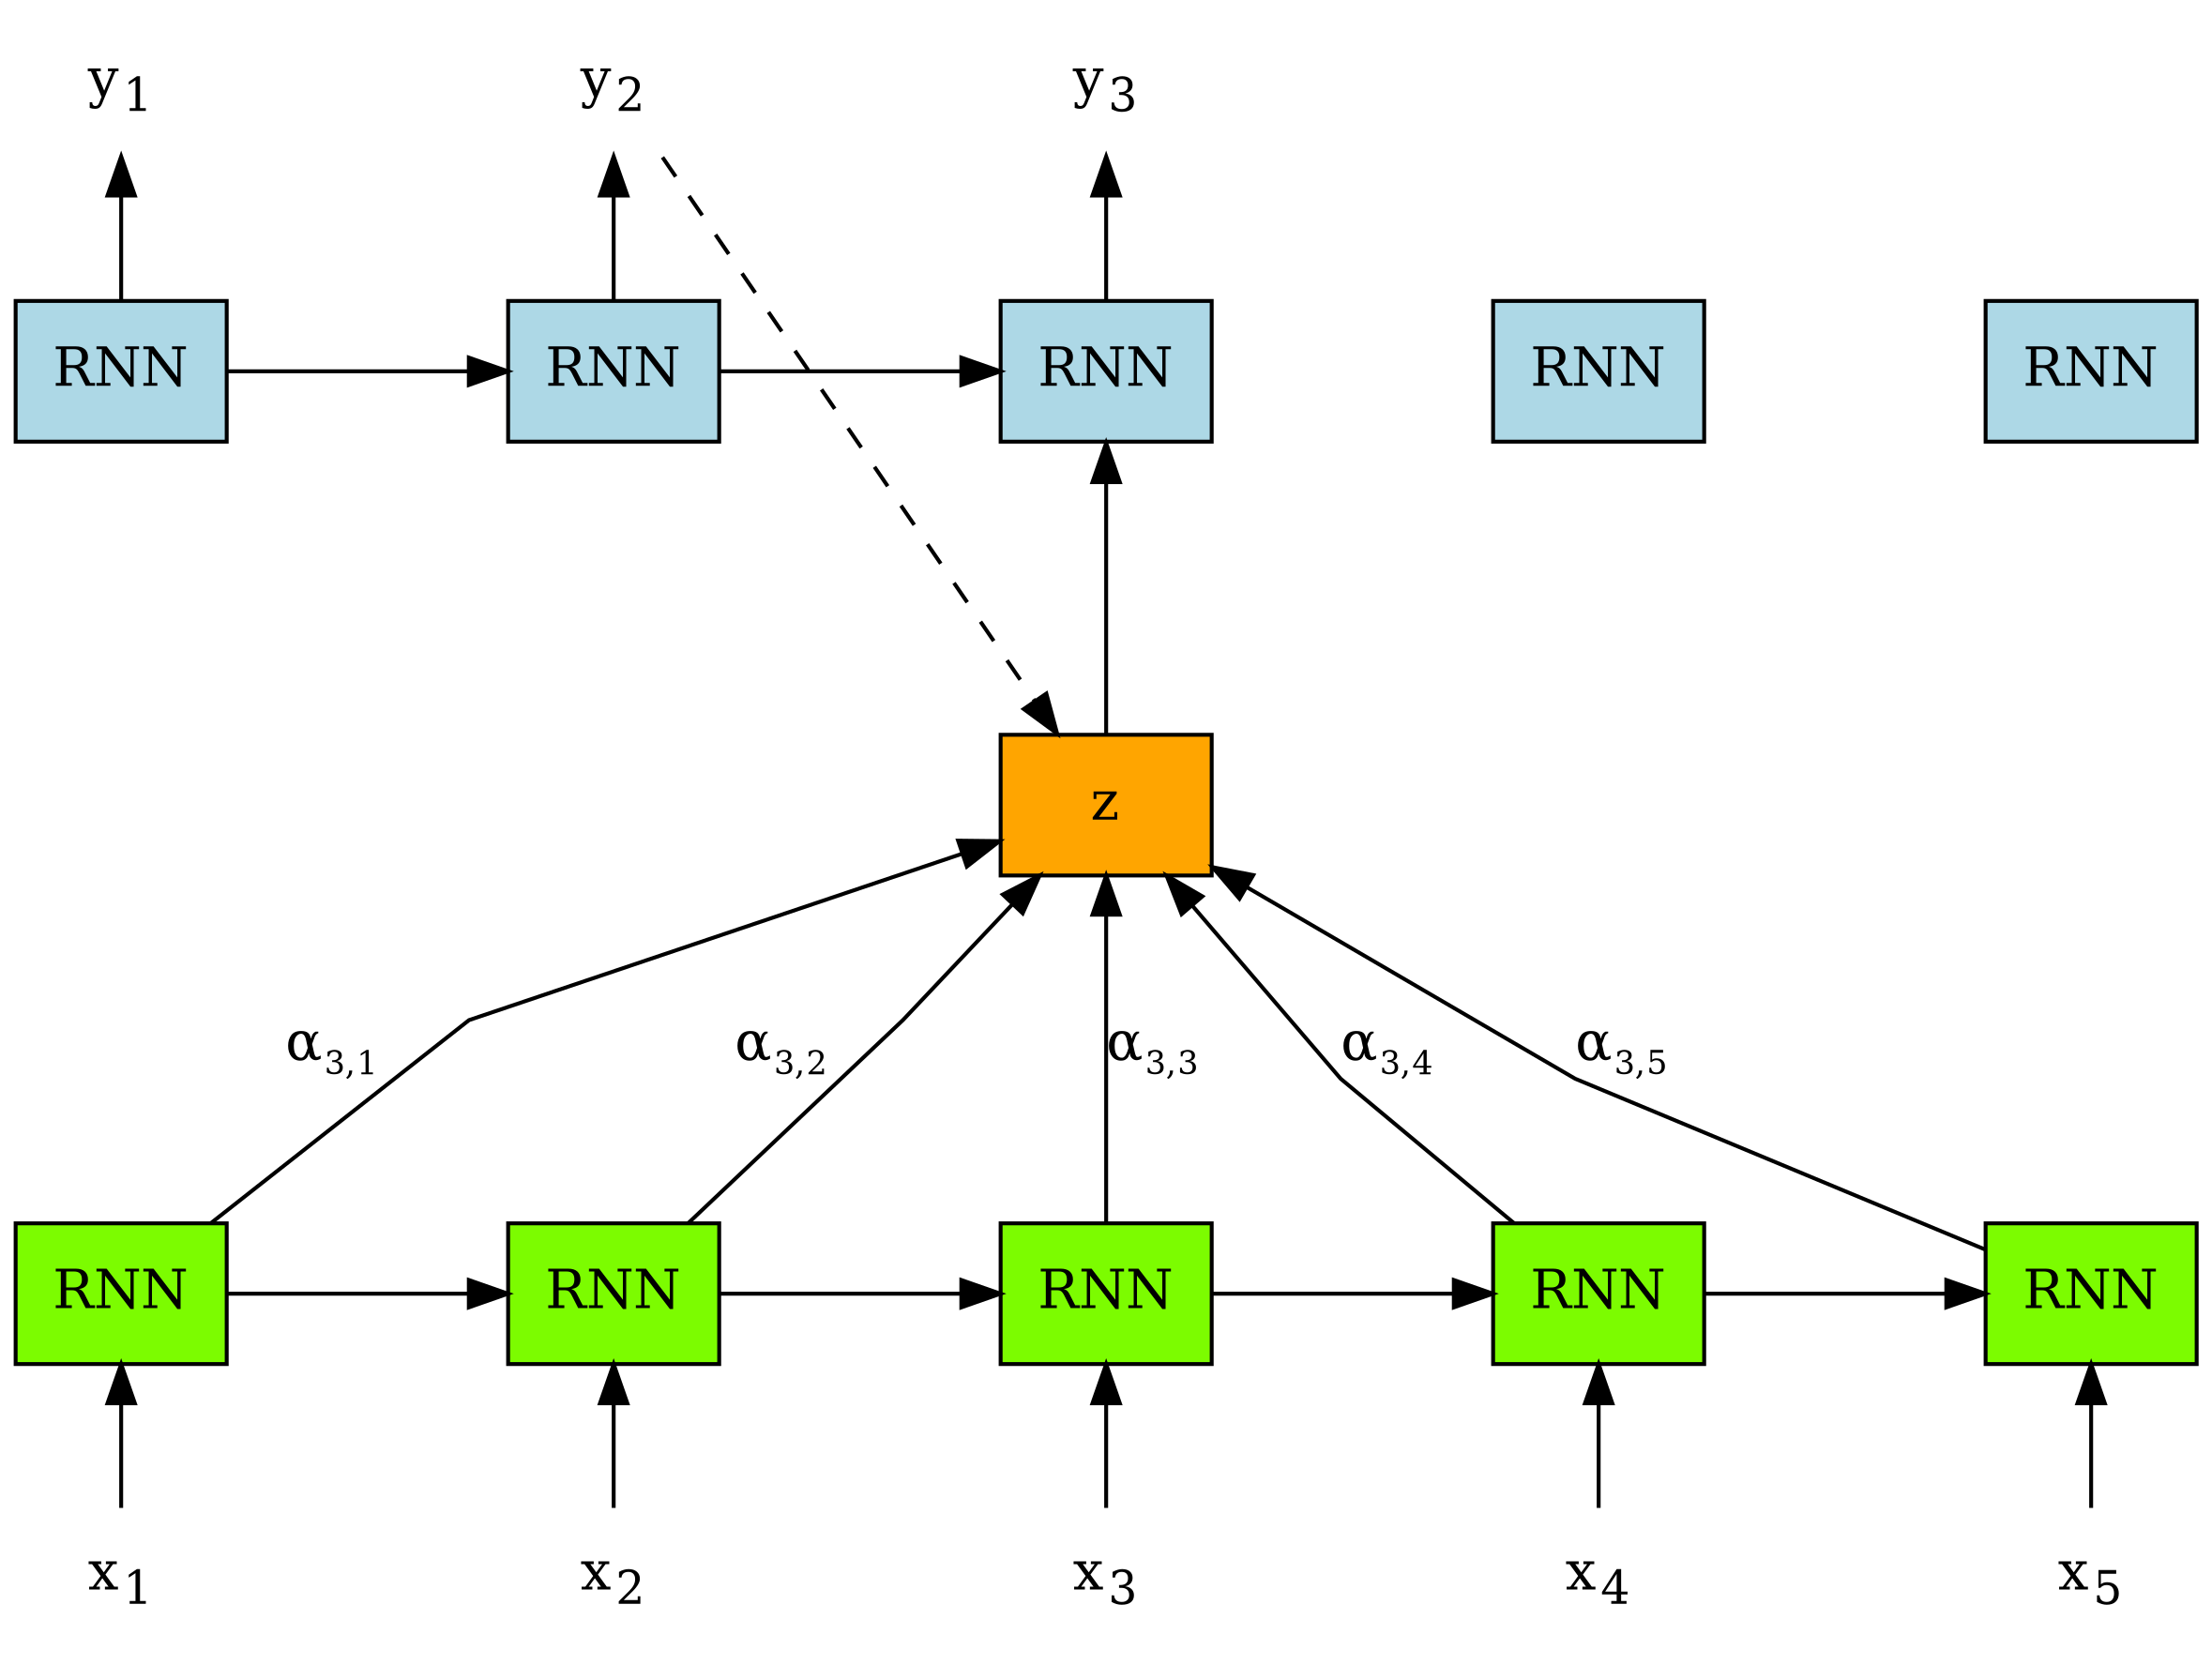
\includegraphics[width=14cm, height=7cm, keepaspectratio]{graphs/transformer_9.png}
\end{center}}
\only<4>{\begin{center}
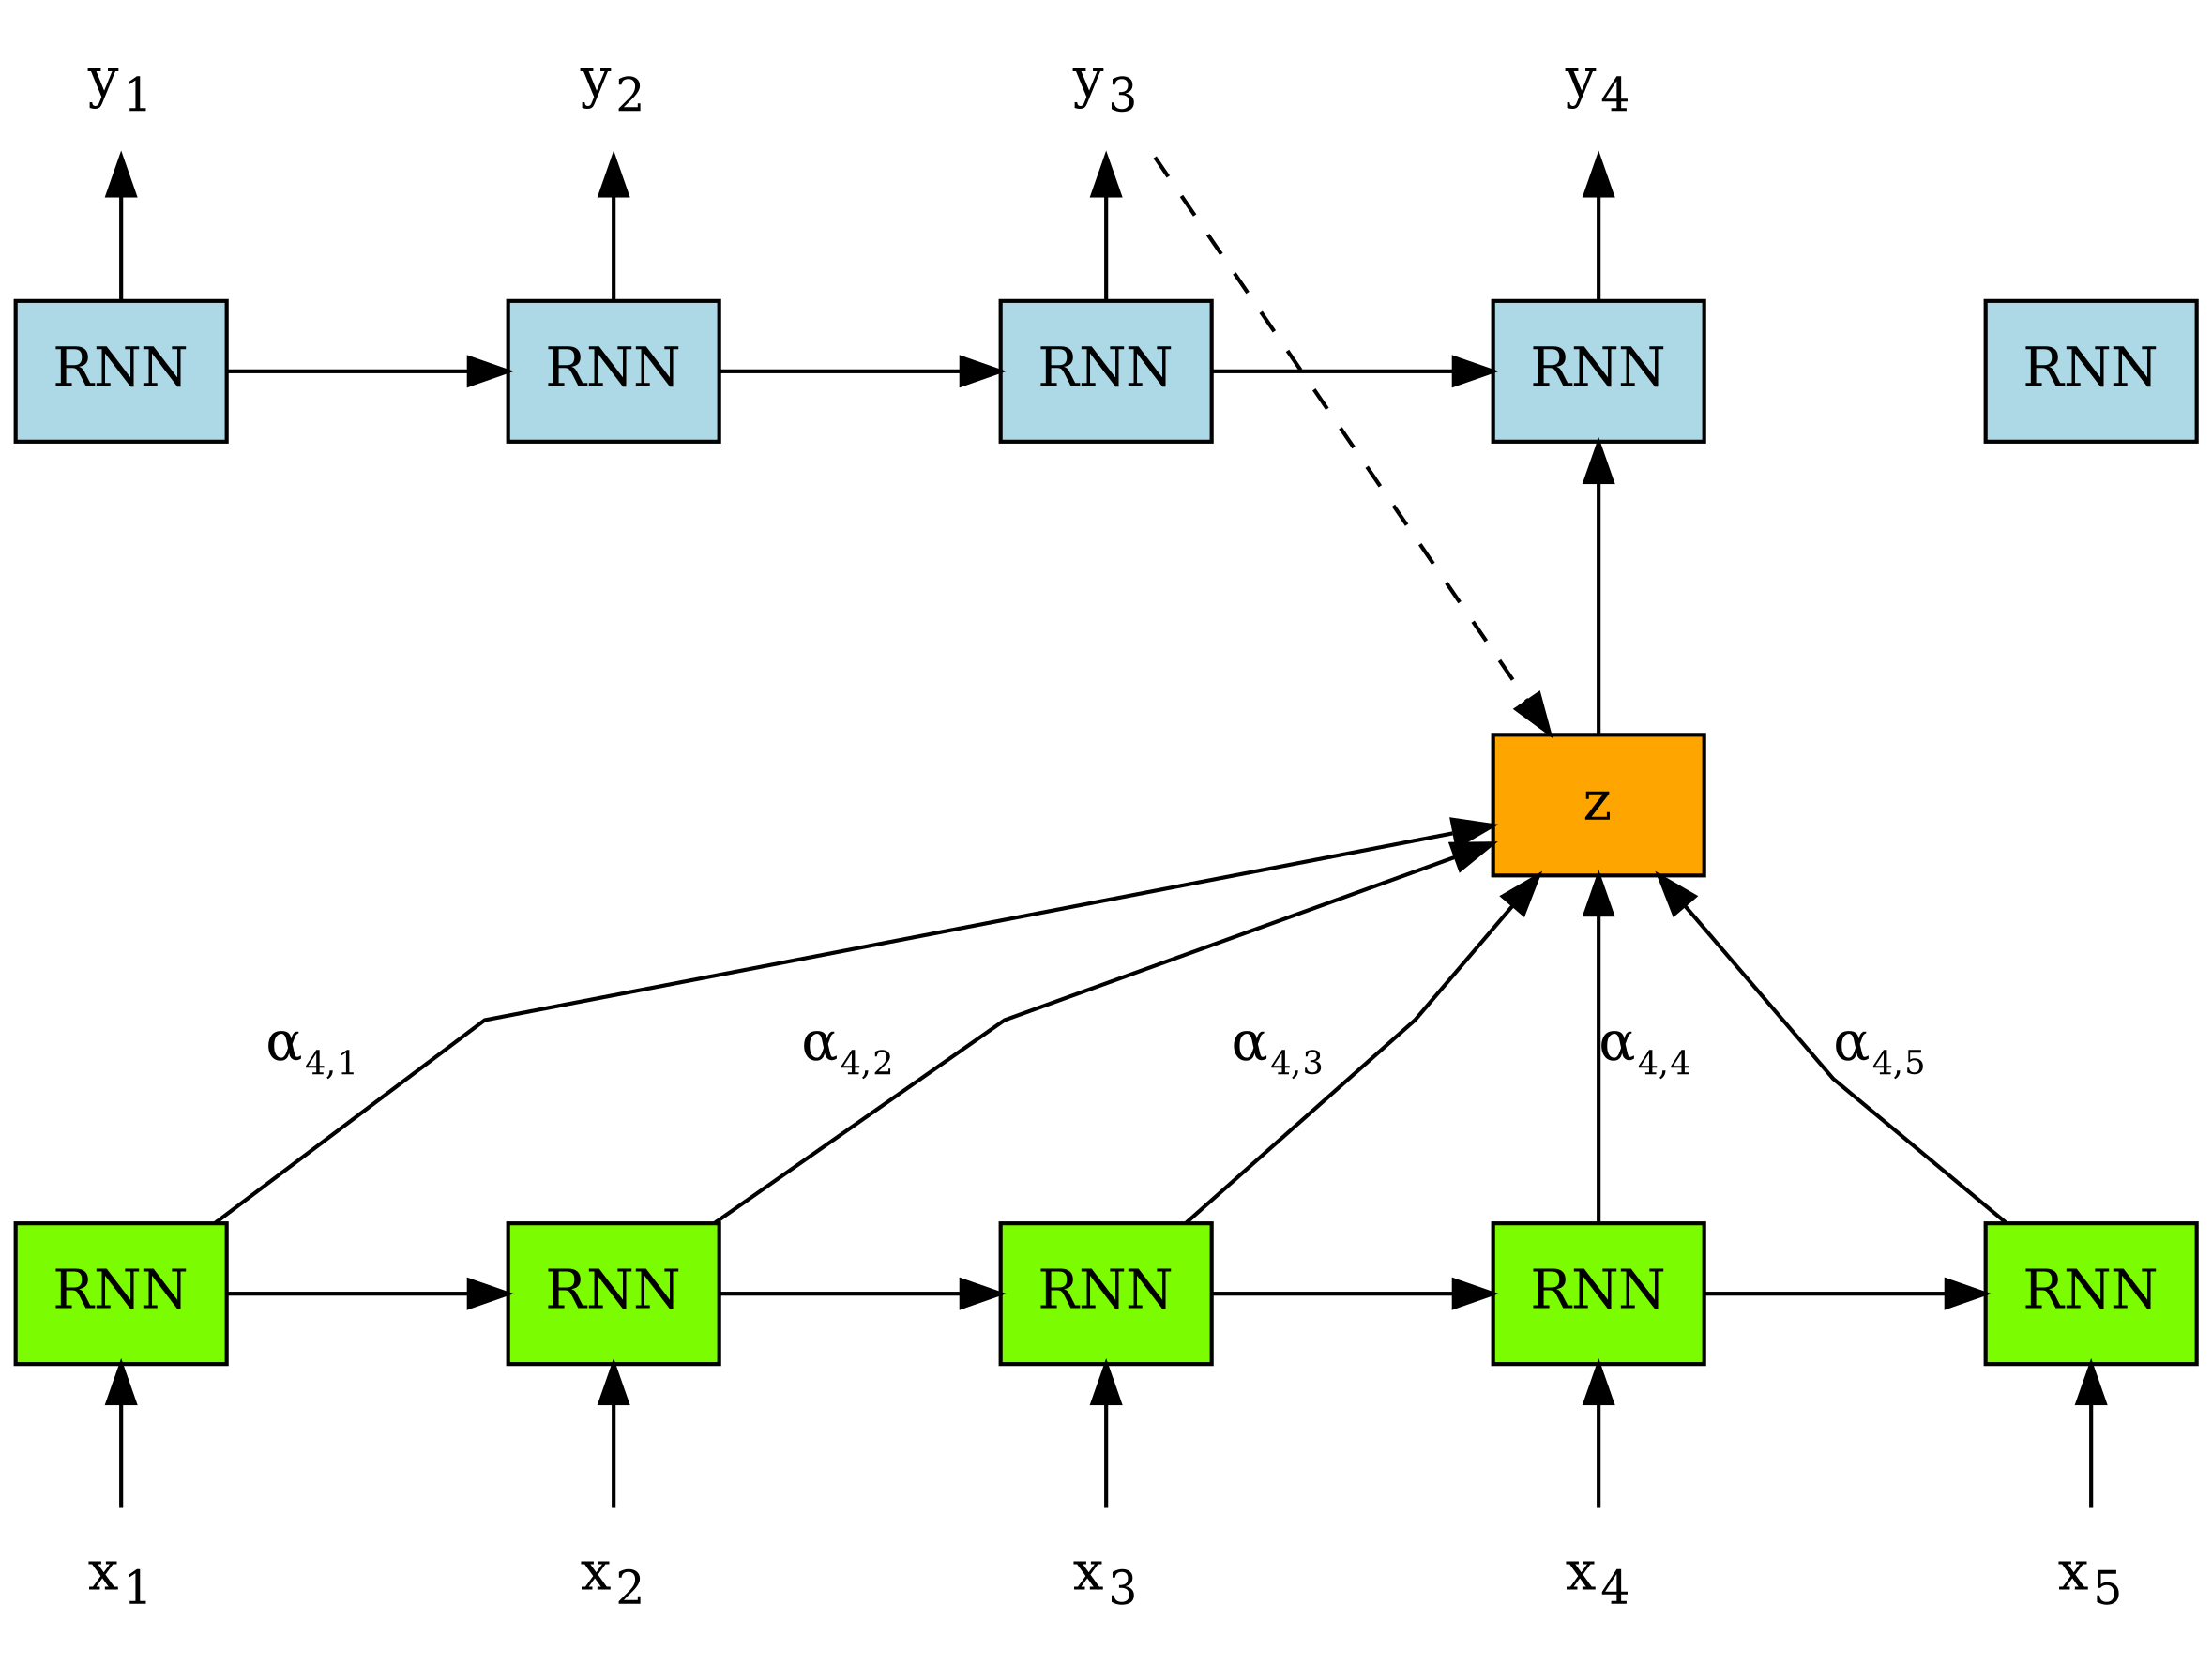
\includegraphics[width=14cm, height=7cm, keepaspectratio]{graphs/transformer_10.png}
\end{center}}
\only<5>{\begin{center}
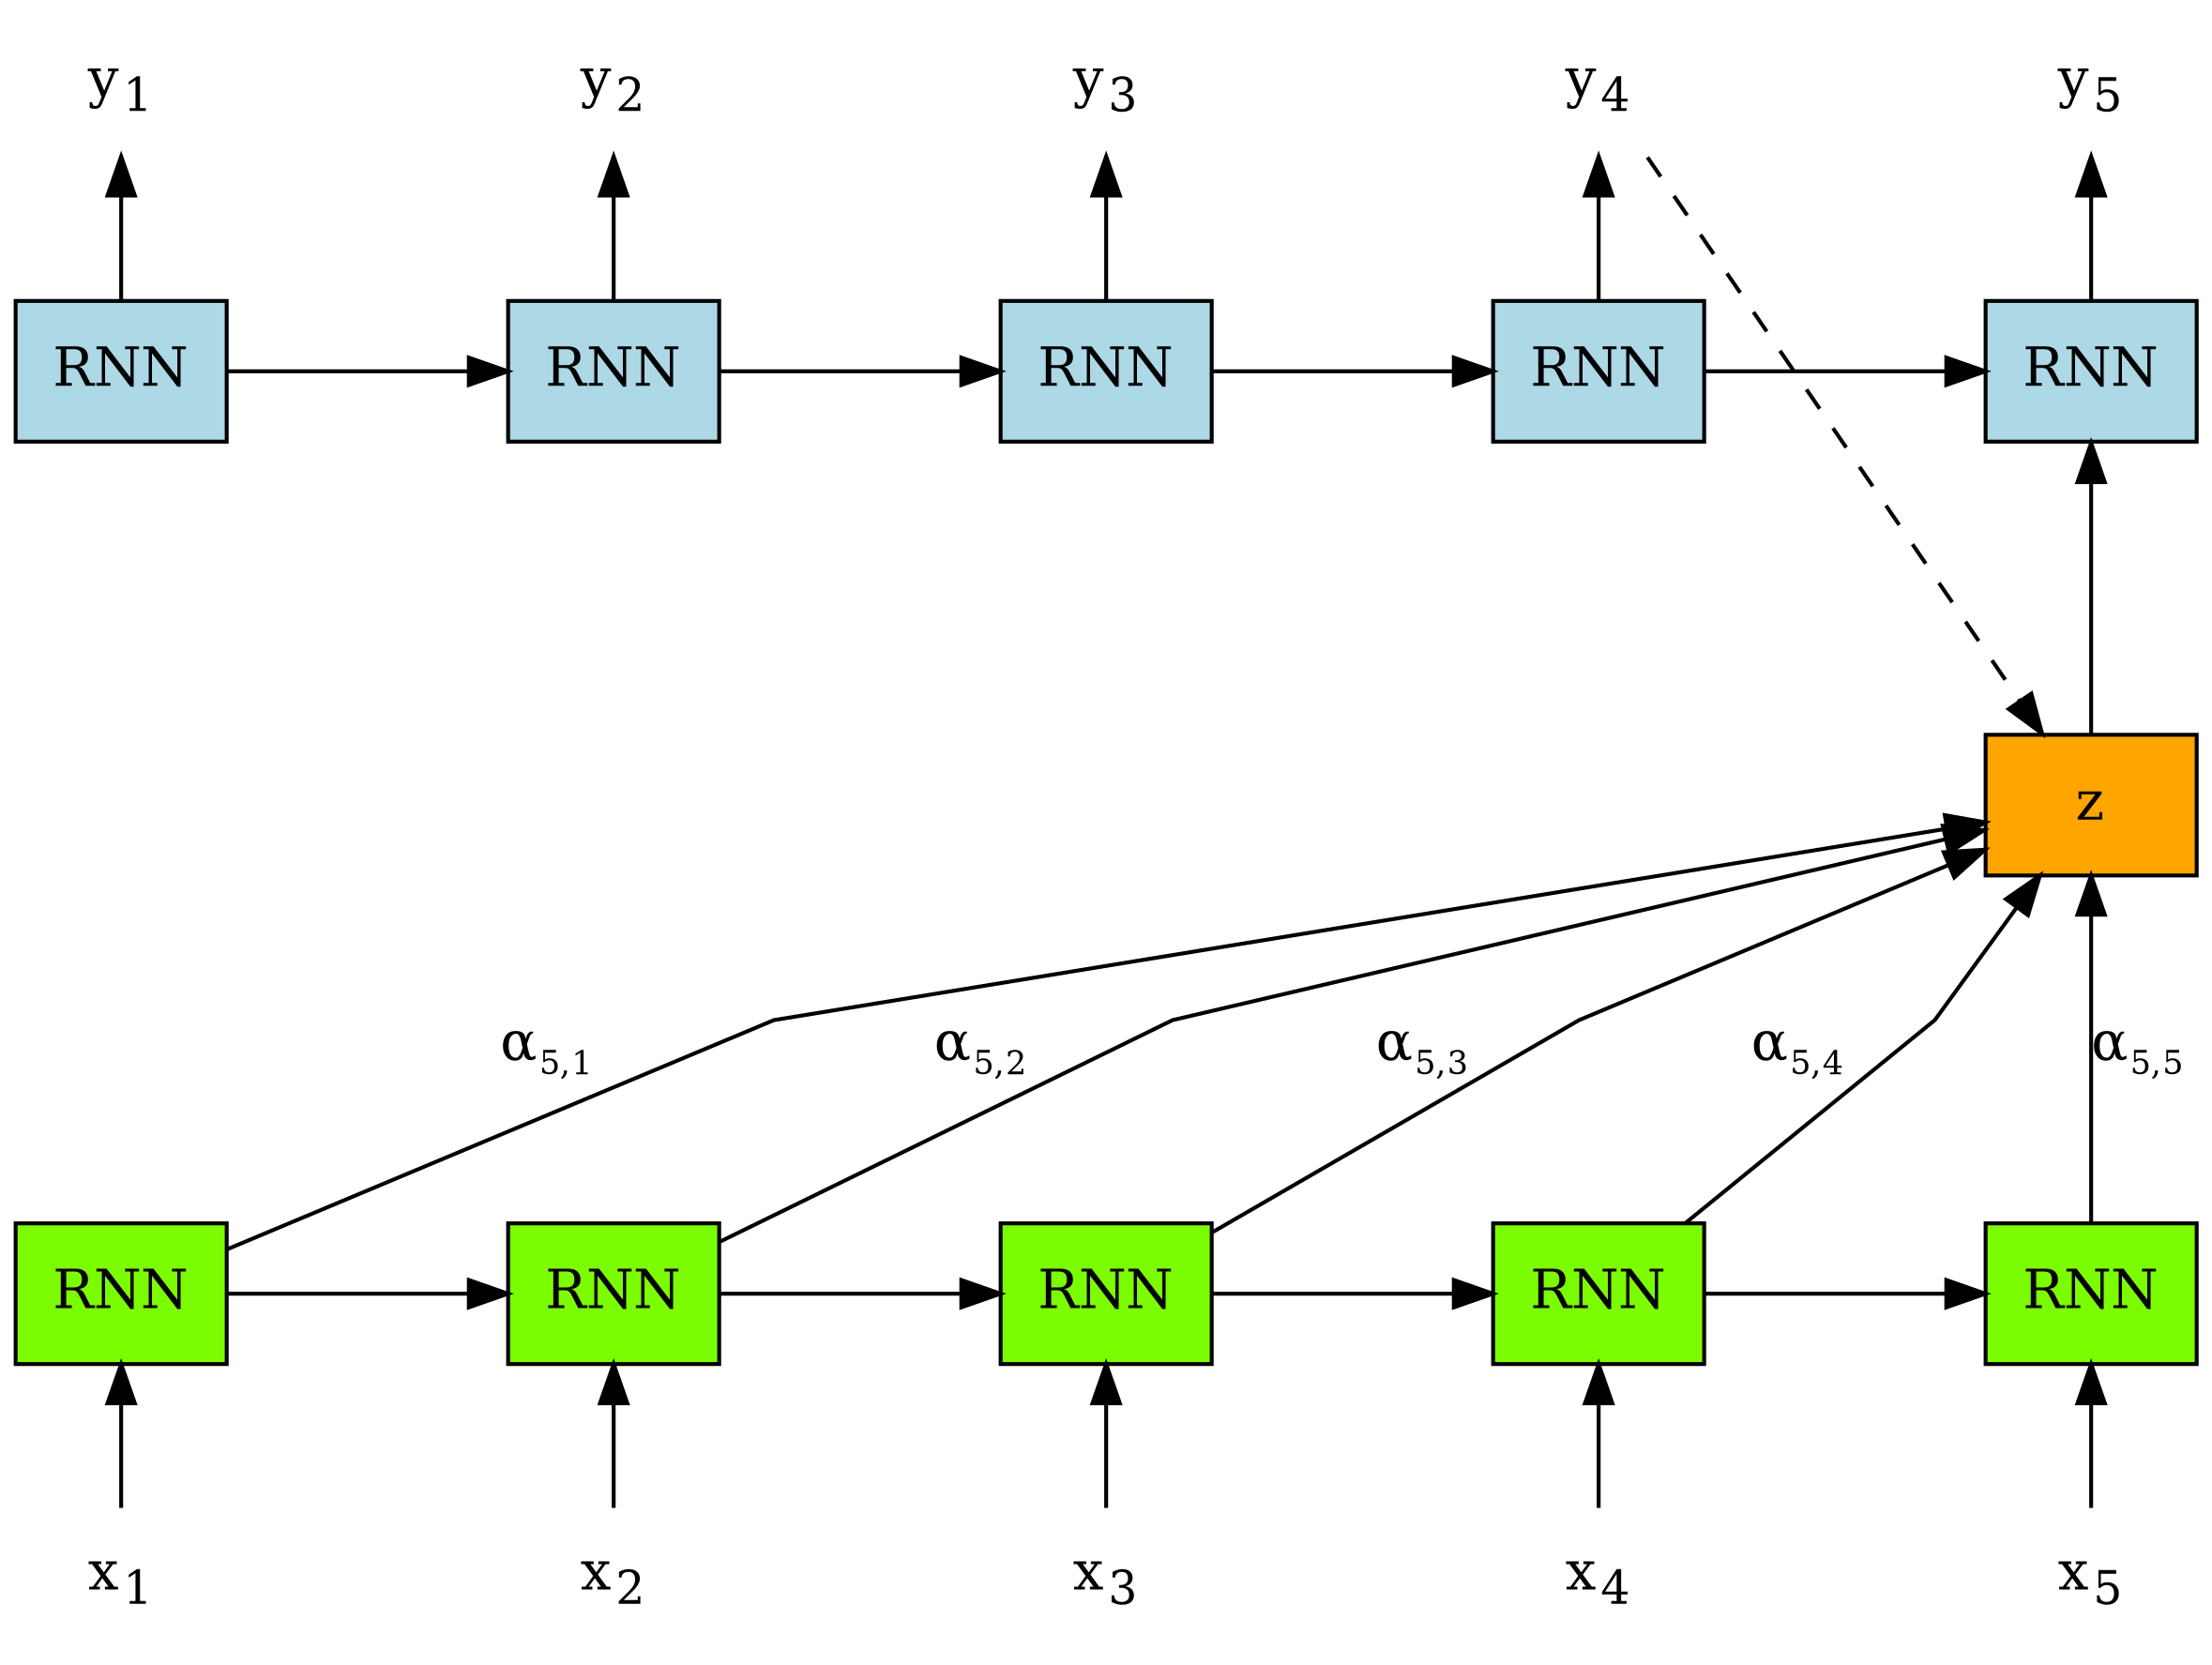
\includegraphics[width=14cm, height=7cm, keepaspectratio]{graphs/transformer_11.png}
\end{center}}
\end{column}
\end{columns}
\end{frame}

\begin{frame}{Figyelmi hőtérkép}
\begin{columns}
\begin{column}{.5\textwidth}
A hőtérkép mutatja, hogy az egyes szavak \textbf{mennyire koncentrálódnak egymásra a fordítási folyamat során}. Ezáltal látható, \textbf{mely szavak között van erős kapcsolat}, és hogyan alakul ki a fordítás folyamata.
\end{column}
\begin{column}{.5\textwidth}
\begin{center}
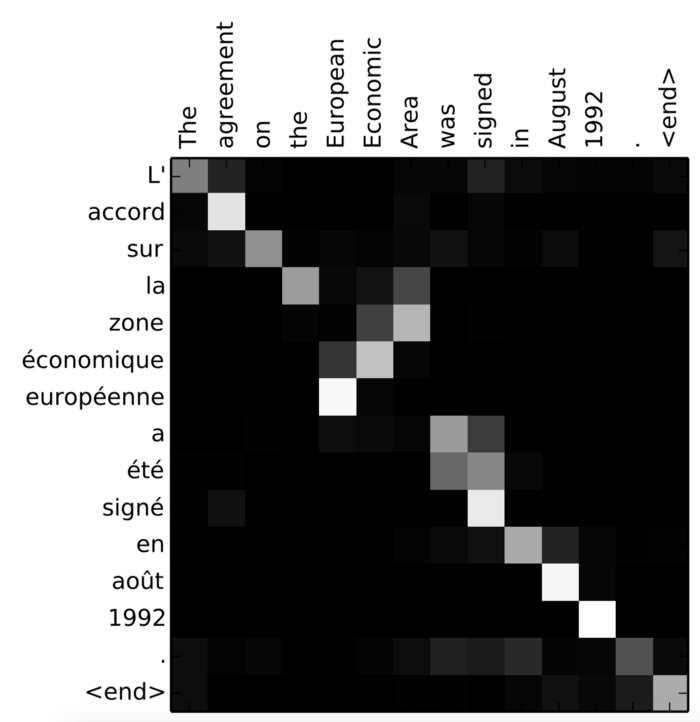
\includegraphics[width=6cm, height=7cm, keepaspectratio]{images/transformer_2.png}
\end{center}
\end{column}
\end{columns}
\end{frame}

\begin{frame}{Jellemzőalapú figyelem}
\begin{columns}
\begin{column}{.5\textwidth}
A kulcs-érték-lekérdezés struktúra a transzformáló architektúrák \textbf{összetett információlekérdezési rendszerének alapjait képezik}.\par\smallskip
Az eljárás mögötti intuíció:
\begin{enumerate}
	\item A modell lekérdezést (\textbf{Q}) intéz a tárolóhoz.
	\item A keresőmotor a lekérdezést kulcsokhoz (\textbf{K}) rendeli, amik megfelelően leírják azt.
	\item Az algoritmus megkeresi a kulcsokra legjobban illeszkedő értékeket (\textbf{V}).
\end{enumerate}
\end{column}
\begin{column}{.5\textwidth}
\begin{center}
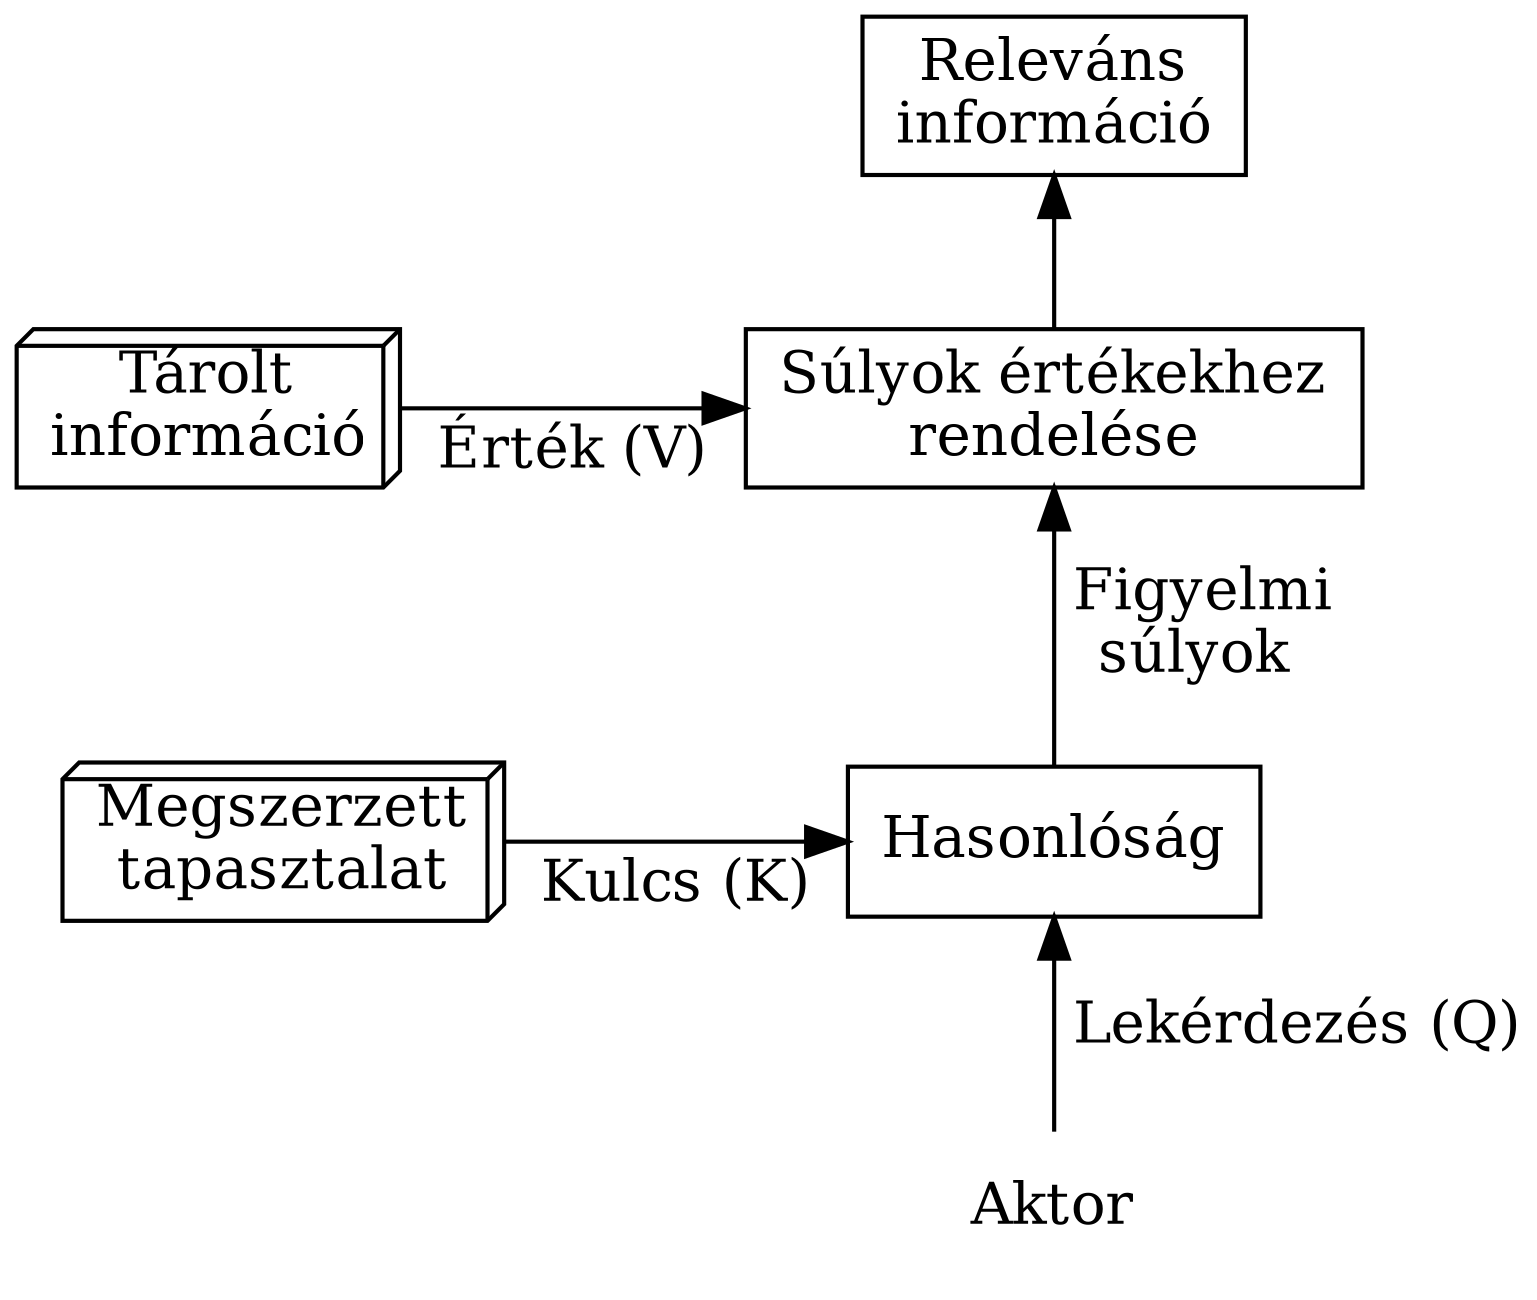
\includegraphics[width=7cm, height=7cm, keepaspectratio]{graphs/transformer_12.png}
\end{center}
\end{column}
\end{columns}
\end{frame}

\begin{frame}{Kulcs-érték-lekérdezés eljárása}
\begin{columns}
\begin{column}{.6\textwidth}
A gyakorlatban a transzformáló 3 különböző reprezentációt használ a lekérdezéseknek, kulcsoknak és értékeknek. A reprezentáció az $X$ beágyazómátrix és $W_q, W_k, W_v$ súlymátrixok szorzataként számolódik ki. Az eredő dimenziószám kevesebb lesz az eredetinél.\par\smallskip
Ezáltal előáll a transzformáló architektúra \textbf{önfigyelem} rétege:
\begin{block}{}
\vspace{-0.4cm}
\[
Figyelem\left( Q,K,V \right) = softmax\left( \frac{Q \cdot K^\intercal}{\sqrt{d_k}}  \right)V
\]
\end{block} 
Ahol $d_k$ a kulcsvektor dimenziószáma.
\end{column}
\begin{column}{.4\textwidth}
\begin{center}
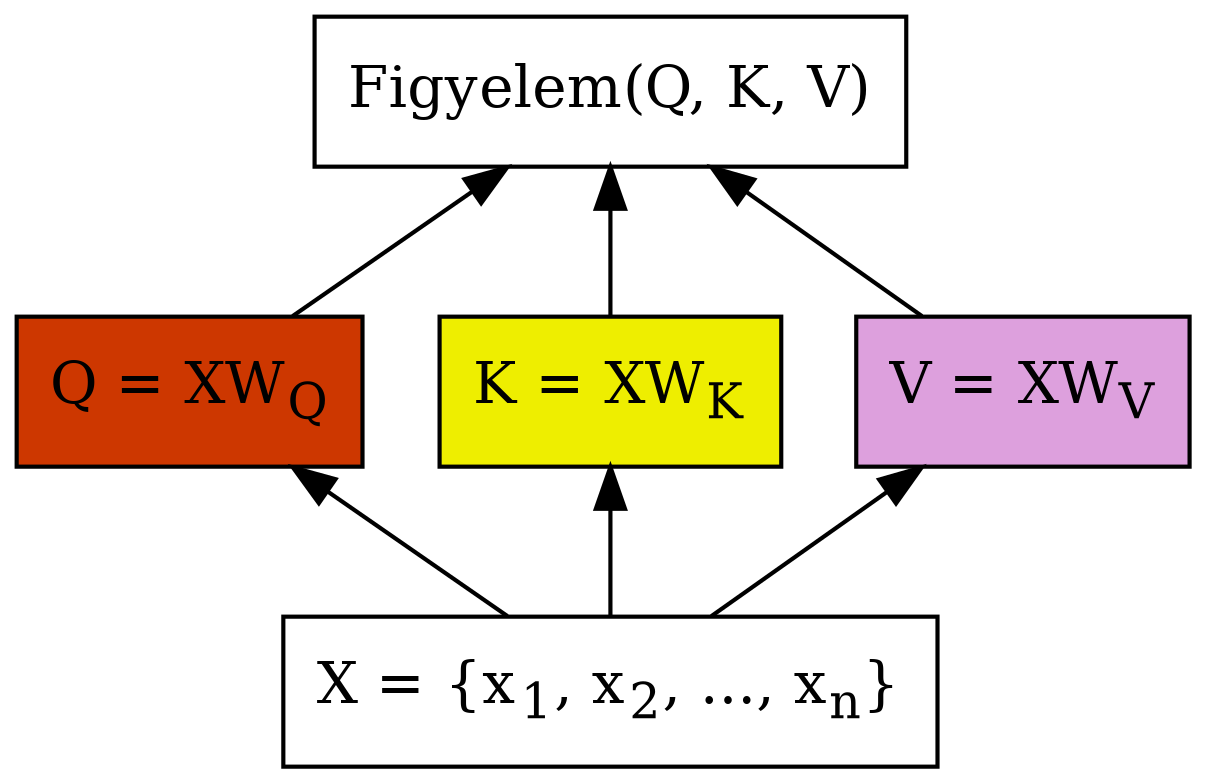
\includegraphics[width=6cm, height=7cm, keepaspectratio]{graphs/transformer_13.png}
\end{center}
\end{column}
\end{columns}
\end{frame}

\begin{frame}{Önfigyelem}
\begin{columns}
\begin{column}{.5\textwidth}
A figyelem nem csak két szekvencia között definiálható, hanem abban az esetben is, \textbf{ha az input és output szekvencia megegyezik}.\par\smallskip
Ez teszi lehetővé a modellnek, hogy a szekvencián belüli elemekhez \textbf{fontossági súlyokat rendeljen}. Így sajátítja el a modell a különböző elemek \textbf{struktúráját és a közöttük lévő kapcsolatokat}.\par\smallskip
A figyelmi reprezentáció minden szóra kiszámolódik:
\begin{block}{}
\vspace{-0.2cm}
\[
A(Q,K,V) = A_1,A_2,\ldots,A_n
\]
\end{block}
\end{column}
\begin{column}{.5\textwidth}
\begin{center}
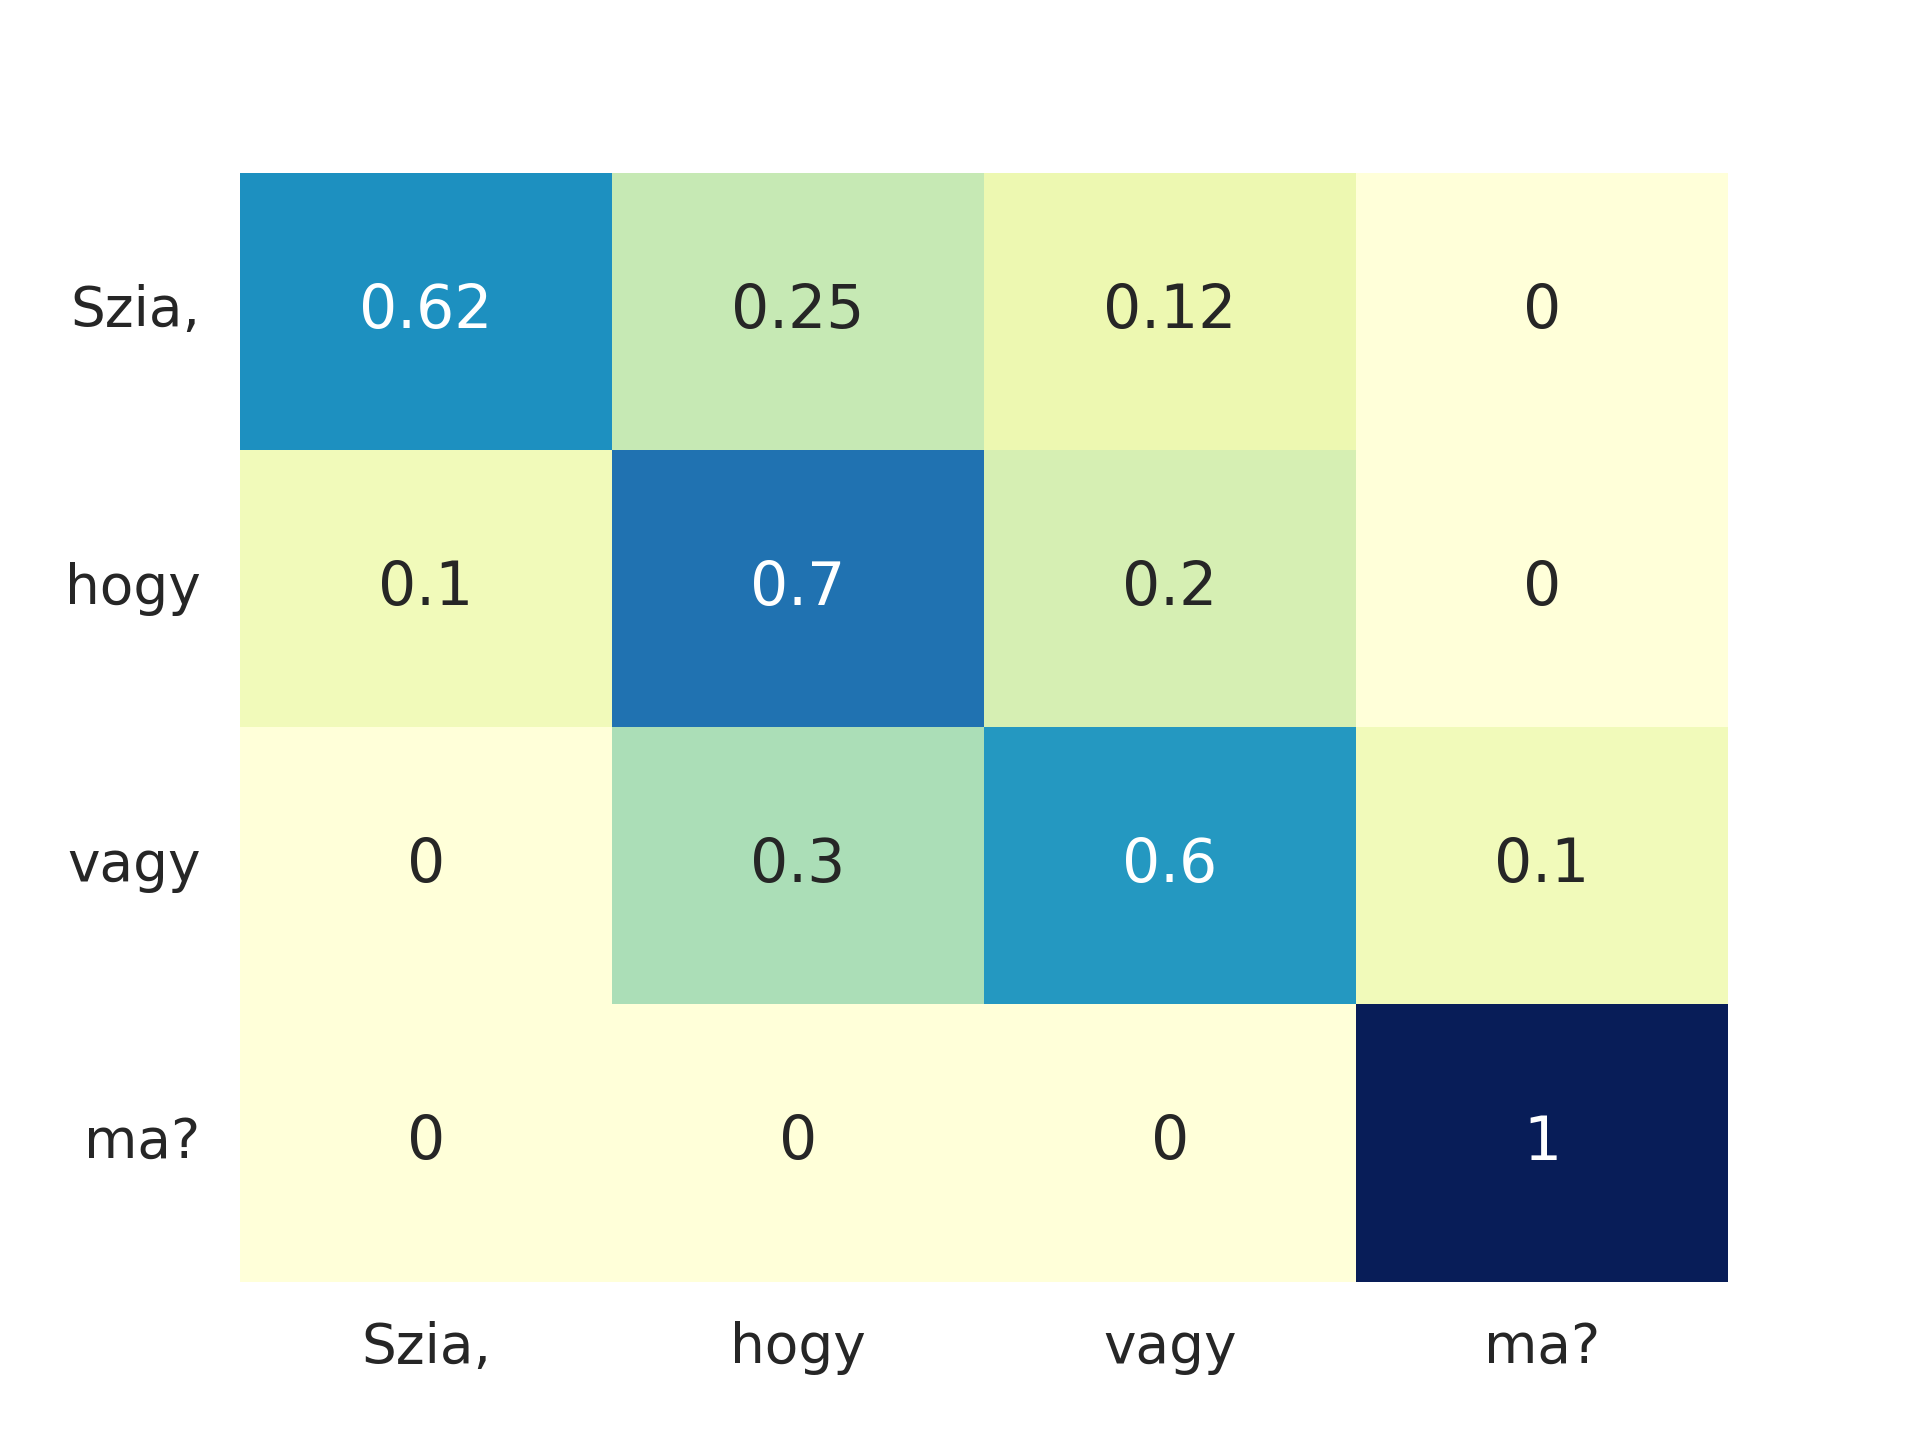
\includegraphics[width=7cm, height=7cm, keepaspectratio]{images/self_attention.png}
\end{center}
\end{column}
\end{columns}
\end{frame}

\end{document}


















